\documentclass{book}
\usepackage{graphicx} % Required for inserting images

\usepackage{mathtools}
\usepackage{listings, xcolor}
\usepackage{color}
\usepackage{geometry}
\usepackage{graphicx}
\usepackage{tikz-qtree}
\usetikzlibrary{arrows}
\usepackage{multirow}
\usepackage{hyperref}

\usepackage{amsmath}
\usepackage{amsfonts}
\usepackage[makeroom]{cancel}

\usepackage{algorithm}
\usepackage[noend]{algpseudocode}
\makeatletter
\def\BState{\State\hskip-\ALG@thistlm}
\makeatother


\newgeometry{
left=   1 in,
bottom= 1.5 in,
right=  1 in,
top=    1 in
}


\title{Advanced Algorithms Notes}
\author{Riccardo Cappi}
\date{February 2024}

\begin{document}

\maketitle

\section{Disclaimer}
These are just my notes that I used to prepare for the exam. So, probably, there will be both spelling and conceptual errors. Feel free to contact me at riccardo.cappi@studenti.unipd.it if you find any errors. This is the github repo where you can find the latex files of the notes: \url{https://github.com/riccardocappi/Computer-Science-notes}

\tableofcontents


\chapter{Lec 01 - Graph Algorithms I}

\section{Graphs: The basis}
A graph is a representation of the relationships between \textbf{pairs} of objects. We denote a graph as follows:
\[G = (V, E)\]
where $V$ is a \textbf{set} of vertices (nodes) and $E$ is a collection of edges. An edge is a pair of vertices $(u, v)$ which indicates the connection between the two nodes.
\begin{itemize}
    \item if $(u, v) = (v, u)$ the graph is \textbf{undirected}
    \item if $(u, v) \neq (v, u)$ the graph is \textbf{directed}
\end{itemize}
In directed graphs an edge is usually called \textit{"arc"}.

Examples of real-world graphs are:
\begin{itemize}
    \item Road networks: $(Cities, Roads)$
    \item Computer networks (e.g. internet): $(Computers, connections)$
    \item World Wide Web: $(Web pages, hyperlinks)$
    \item Social networks: $(People, friendship \,\, connections)$
\end{itemize}

\section{Terminology}
\begin{itemize}
    \item Given an edge $e = (u, v)$, $e$ is \textbf{incident} on $u$ and $v$, while $u, v$ are \textbf{adjacent}.

    \item The \textbf{neighbors} of a vertex $u$ are all the vertices $v$ such that $(u, v) \in E$. 

    \item The \textbf{degree} of a vertex $d(v)$ is the number of edges incident on $v$.
\end{itemize}

\section{Concepts}
\begin{itemize}
    \item \textbf{Simple path}: A sequence of nodes $v_{1}, v_{2}, ..., v_{k}$ all distinct such that $(v_{i}, v_{i + 1}) \in E \,\, \forall 1 \leq i < k$. Having all distinct nodes makes the path a simple path. 

    \item \textbf{Cycle}: is a path such that $v_{1} = v_{k}$

    \item \textbf{Sub-graph:} $G' = (V', E')$ such that $V' \subseteq V, \,\, E' \subseteq E$ and the edges of $E'$ are incident only on $V'$.

    \item \textbf{Spanning sub-graph:} a sub-graph with $V' = V$

    \item \textbf{Connected graph:} a graph is connected if $\forall u, v \in V$ it exists a path from $u$ to $v$.

    \item \textbf{Connected components:} a partition of $G$ in sub-graphs $G_{i} = (V_{i}, E_{i})$ such that $\forall 1 \leq i < k$ 
    \begin{itemize}
        \item $G_{i}$ is connected.
        \item $V$ = $V_{1} \cup V_{2} \cup ... \cup V_{k}$
        \item $E = E_{1} \cup E_{2} \cup... \cup E_{k}$
        \item $\forall i \neq j$ there is no edge between $V_{i}$ and $V_{j}$
    \end{itemize}
    If $G$ is connected, then $k = 1$.

    \item \textbf{Tree:} connected graph without cycles.

    \item \textbf{Forest:} set of trees (disjoint)

    \item \textbf{Spanning tree:} a spanning connected sub-graph without cycles (it exists only if $G$ is connected).

    \item \textbf{Spanning forest:} a spanning sub-graph without cycles.
\end{itemize}

\section{Basic problems}
\begin{itemize}
    \item Traversal
    \item Connectivity (tell if the graph is connected or not)
    \item Compute connected components
    \item Minimum-weight spanning trees
    \item Shortest paths
    \item ...
\end{itemize}

\section{Notations and Properties}
\begin{itemize}
    \item $n = |V|$
    \item $m = |E|$
    \item The \textbf{size} of the graph is given by $n + m$
    \item $\sum_{v \in V}d(v) = 2m$ because in the summation every edge counts twice.
    \item $m \leq \binom{n}{2}$
    \item if $G$ is a tree $m = n - 1$ because, fixed a root, $E$ represents father-child similarities, which are $n - 1$.
    \item if $G$ is connected $m \geq n - 1$ because $G$ is a \textit{"tree"} that may have cycles, thus it can only have more edges.
    \item if $G$ is acyclic $m \leq n - 1$ because $G$ is a tree that may not be connected, thus it can only have less edges.
\end{itemize}


\chapter{Lec 02 - Problem Solving Agent}
\section{Solving Problems by Searching}
We'll describe one kind of \textbf{goal-based} agent called a problem-solving agent. Our discussion of problem solving begins with precise definitions of \textbf{problems} and their \textbf{solutions} and give several examples to illustrate these definitions. We then describe several
general-purpose search algorithms that can be used to solve these problems. We will see several \textbf{uninformed} search algorithms, algorithms that are given no information about the problem other than its definition. Let's start with an example:\newline\newline
Imagine an agent in the city of Arad, Romania, enjoying a touring holiday. Now, suppose the agent has a nonrefundable ticket to fly out of Bucharest the following day. In that case, it makes sense for the agent to adopt the \textbf{goal} of getting to Bucharest by driving across various cities. Therefore, the \textbf{problem formulation} can be defined as follows:
\begin{itemize}
    \item Formulate goal: be in Bucharest
    \item Formulate problems:
    \begin{itemize}
        \item states: various cities
        \item actions: drive between cities
    \end{itemize}
    \item Solution: sequence of cities; e.g. Arad, Sibiu, Fagaras, Bucharest
\end{itemize}
\begin{center}
    \includegraphics[scale=0.8]{images/Romania.png}
\end{center}
We assume that the environment is \textbf{observable}, so the agent always knows the current state. For the agent driving in Romania, it’s reasonable to suppose that each city on the map has a sign indicating its presence to arriving drivers. We also assume the environment is \textbf{discrete}, so at any given state there are only finitely many actions to choose from. This is true for navigating in Romania because each city is connected to a small number of other cities. We will assume the environment is \textbf{known}, so the agent knows which states are reached by each action. (Having an accurate map suffices to meet this condition for navigation problems.) Finally, we assume that the environment is \textbf{deterministic}, so each action has exactly one outcome.\newline\newline
The process of looking for a sequence of actions that reaches the goal is called \textbf{search}. A search algorithm takes a problem as input and returns a \textbf{solution} in the form of an action sequence.
\begin{center}
    \includegraphics[scale=0.8]{images/problem-solving agent.png}
\end{center}
A problem can be defined formally by four components:
\begin{itemize}
    \item The \textbf{initial state} that the agent starts in. For example, the initial state for our agent in Romania might be described as \textit{In(Arad)}.

    \item A description of what each action does; the formal name for this is the \textbf{transition model}. We also use the term \textbf{successor} to refer to any state reachable from a given state by a single action. This can be described by a set $E(x)$ of action-state pairs, e.g. $E(In(Arad)) = \{<Arad \rightarrow Zerind, Zerind>, ...\}$. An alternative formulation for the successor function can be the actions that can be performed in a given state.

    \item The \textbf{goal test}, which determines whether a given state is a goal state. The goal can be explicit, e.g. the singleton set \footnote{There can be multiple goal states} $\{In(Bucharest)\}$, or implicit, an abstract property rather than an explicitly enumerated set of states.

    \item A \textbf{path cost} function that assigns a numeric cost to each path. The problem-solving agent chooses a cost function that reflects its own performance measure. For the agent trying to get to Bucharest, time is of the essence, so the cost of a path might be its length in kilometers. The \textbf{step cost} of taking action $a$ in state $s$ to reach state $s'$ is denoted by $c(s, a, s')$, assumed to be $\geq 0$.
\end{itemize}
The preceding elements define a problem and can be gathered into a single data structure that is given as input to a problem-solving algorithm. A solution to a problem is an action sequence that leads from the initial state to a goal state. Solution quality is measured by the path cost function, and an \textbf{optimal solution} has the lowest path cost among all solutions.

\section{Selecting a State Space}
Real world is absurdly complex. Compare the simple state description we have chosen, $In(Arad)$, to an actual crosscountry trip, where the state of the world includes so many things: the traveling companions, the current radio program, the scenery out of the window, the proximity of law enforcement officers, etc. All these considerations are left out of our state descriptions because they are irrelevant to the problem of finding a route to Bucharest. The process of removing detail from a representation is called \textbf{abstraction}.
\newline\newline
In addition to abstracting the state description, we must abstract the actions themselves.\newline\newline
Now consider a solution to the abstract problem: for example, the path from Arad to Sibiu to Rimnicu Vilcea to Pitesti to Bucharest. This abstract solution corresponds to a large number of more detailed paths.
\newline\newline
The choice of a good abstraction thus involves removing as much detail as possible while retaining validity and ensuring that the abstract actions are easy to carry out.

\section{Searching for Solutions}
A solution is an action sequence, so search algorithms work by considering various possible action sequences. The possible action sequences starting at the initial state form a \textbf{search tree} with the initial state at the root; the branches are actions and the \textbf{nodes} correspond to states in the \textbf{state space} of the problem.
\begin{center}
    \includegraphics[scale=0.8]{images/search tree.png}
\end{center}
We start from the root and, at each step, we need to check whether we reached the goal state. Then, we need to consider taking various actions. We do this by \textbf{expanding} the current state, that is, applying each legal action to the current state, thereby \textbf{generating} a new set of states. In the case of the figure above, we add three branches from the parent node $In(Arad)$ leading to three new child nodes: $In(Sibiu)$, $In(Timisoara)$, and $In(Zerind)$. Now we must choose which of these three possibilities to consider further.\newline\newline
This is the essence of search, following up one option now and putting the others aside for later. The set of all leaf nodes available for expansion at any given point is called the \textbf{frontier}. The process of expanding nodes on the frontier continues until either a solution is found or there are no more states to expand.
\begin{center}
    \includegraphics[scale=0.8]{images/tree search2.png}
\end{center}
Search algorithms all share the basic structure above; they vary primarily according to how they choose which state to expand next, the so-called search strategy.\newline\newline
In the figure representing the search tree of the \textit{driving through Romania} problem we can notice that it includes the path from Arad to Sibiu and back to Arad again. We say that $In(Arad)$ is a \textbf{repeated state} in the search tree, generated in this case by a \textbf{loopy path}.\newline\newline
The way to avoid exploring redundant paths is to remember where one has been. To do this, we augment the TREE-SEARCH algorithm with a data structure called the \textbf{explored set} (also known as the closed list), which remembers every expanded node. Newly generated nodes
that match previously generated nodes can be discarded instead of being added to the frontier. This new algorithm is called GRAPH-SEARCH.\newline\newline
Clearly, the search tree constructed by the GRAPH-SEARCH algorithm contains at most one copy of each state, so we can think of it as growing a tree directly on the state-space graph. Furthermore, the frontier \textbf{separates} the state-space graph into the explored region and the unexplored region, so that every path from the initial state to an unexplored state has to pass through a state in the frontier.\newline\newline
Up to now, we have not been very careful to distinguish between nodes and states, but in writing detailed algorithms it’s important to make that distinction. A node is a bookkeeping data structure used to represent the search tree. It includes \textit{parent, children, depth, path cost}. A state corresponds to a configuration of the
world. Thus, nodes are on particular paths whereas states are not. Furthermore, two different nodes can contain the same world state if that state is generated via two different search paths.\newline\newline
Now that we have nodes, we need somewhere to put them. The frontier needs to be stored in such a way that the search algorithm can easily choose the next node to expand according to its preferred strategy. The appropriate data structure for this is a \textbf{queue}.

\section{Uninformed Search Strategies}
Uniformed Search Strategies include the following:
\begin{itemize}
    \item \textbf{Breadth-first search:} Breadth-first search is a simple strategy in which the root node is expanded first, then all the successors of the root node are expanded next, then their successors, and so on. In general, all the nodes are expanded at a given depth in the search tree before any nodes at the next level are expanded. The frontier is implemented using a FIFO queue.

    \item \textbf{Uniform-cost search:} The idea is to expand least-cost unexpanded node. This is done by storing the frontier as a priority queue ordered by path cost.

    \item \textbf{Depth-first search:} Depth-first search always expands the deepest node in the current frontier of the search tree. the frontier is implemented as a LIFO queue.

    \item \textbf{Iterative deepening depth-first search:} Iterative deepening search (or iterative deepening depth-first search) which repeatedly applies depth first search limiting the depth of the tree. It does this by gradually increasing the limit, first 0, then 1, then 2, and so on, until a goal is found.

    \item \textbf{Bidirectional search:} The idea behind bidirectional search is to run two simultaneous searches—one forward from the initial state and the other backward from the goal—hoping that the two searches meet in the middle.

\end{itemize}
We can evaluate an algorithm’s performance in four ways:
\begin{itemize}
    \item \textbf{Completeness:} Is the algorithm guaranteed to find a solution when there is one?

    \item \textbf{Optimality:} Does the strategy find the optimal solution in terms of cost?

    \item \textbf{Time complexity:} How long does it take to find a solution?

    \item \textbf{Space complexity:} How much memory is needed to perform the search?
\end{itemize}
The evaluation of the previously presented strategies is the following:
\begin{center}
    \includegraphics[]{images/evaluation.png}
\end{center}
where:
\begin{itemize}
    \item $b$ is the branching factor (how many successor a node has)

    \item $d$ is the depth of the shallowest solution

    \item $m$ is the maximum depth of the search tree

    \item $l$ is the depth limit
\end{itemize}
We can easily see that \textbf{Breadth-first search} is complete; if the shallowest goal node is at some finite depth $d$, breadth-first search will eventually find it after generating all shallower nodes. Note that as soon as a goal node is generated, we know it is the shallowest goal node because all shallower nodes must have been generated already
and failed the goal test. However, the shallowest goal node is not necessarily the optimal one. Furthermore, every node generated remains in
memory, making the space complexity $O(b^d)$\newline\newline
On the other hand, \textbf{Uniform-cost search} is optimal in general. First, we observe that whenever uniform-cost search selects a node $n$ for expansion, the optimal path to that node has been found. Then,
because step costs are non-negative, paths never get shorter as nodes are added.\newline\newline
The properties of \textbf{depth-first search} depend strongly on whether the graph-search or tree-search version is used. The graph-search version, which avoids repeated states and redundant paths, is complete in finite state spaces because it will eventually expand every node. The tree-search version, on the other hand, is not complete (it may get stuck in a loop). The time complexity of depth-first tree search is $O(b^m)$. Note that $m$ itself can be much larger than $d$. So far, depth-first search seems to have no clear advantage over breadth-first search, so why do we include it? The reason is the space complexity. For a graph search, there is no advantage, but a depth-first tree search needs to store only a single path from the root to a leaf node, along with the remaining unexpanded sibling nodes for each node on the
path. Once a node has been expanded, it can be removed from memory as soon as all its descendants have been fully explored.\newline\newline
We can combine the completeness of BFS and the space saving of DFS with the \textbf{Iterative deepening search}. This strategy may seem wasteful because states are generated multiple times. It turns out this is not too costly. The reason is that in a search tree with the same (or nearly the same) branching factor at each level, most of the nodes are in the bottom level, so it does not matter much that the upper levels are generated multiple times.\newline\newline



\chapter{Lec 03 - From DFS to BFS}

\section{More applications of DFS}
DFS can also be used to solve the following 2 problems:
\begin{itemize}
    \item Connected Components: Labelling all the vertices of $G$ such that 2 vertices have the same label iff they are in the same connected components.
    \item Connectivity: Return whether the graph is connected or not. 
\end{itemize}

\subsection{Connected Components}
\begin{algorithm}
\caption{ConnectedComponents}\label{Conn.Comp.}
    \begin{algorithmic}[1]
    \Procedure{ConnectedComp ($G$)}{}
        \For{$v \gets 1$ to $n$}
            \State $L_{V}[v].ID = 0$
        \EndFor
        \State $k \gets 0$
        \For{$v \gets 1$ to $n$}
            \If{$L_{V}[v].ID = 0$}
                \State $k \gets k + 1$
                \State DFS($G, v, k$)
            \EndIf
        \EndFor
    \EndProcedure
    \end{algorithmic}
\end{algorithm}
We have to modify the DFS algorithm in such a way that $L_{V}[v] \gets k$. The $ID$ field of each node is no more either 0 or 1, but it corresponds to the ID of the $k$-th connected component. 

\subsection{Connectivity}
\begin{algorithm}
\caption{Connectivity}\label{Connectivity}
    \begin{algorithmic}[1]
    \Procedure{Connectivity ($G$)}{}
        \For{$v \gets 1$ to $n$}
            \State $L_{V}[v].ID = 0$
        \EndFor
        \State $k \gets 0$
        \For{$v \gets 1$ to $n$}
            \If{$L_{V}[v].ID = 0$}
                \State $k \gets k + 1$
                \State DFS($G, v, k$)
            \EndIf
        \EndFor
        \State \textbf{if} $k = 1$ \textbf{return} $Yes$ \textbf{else} $False$
    \EndProcedure
    \end{algorithmic}
\end{algorithm}
The algorithm is similar to the one used for computing the connected components, but in this case we return if the graph is connected or not ($k = 1$).\newline\newline
The complexity of both algorithms is $\Theta(n + m)$.

\section{Summary}
Given a graph $G = (V, E)$, the following problems can be solved using DFS:
\begin{itemize}
    \item Test if $G$ is connected.
    \item Find the connected components of $G$.
    \item Find a spanning tree of $G$ (if $G$ is connected).
    \item Find a path between 2 vertices (if any).
    \item Find a cycle (if any).
\end{itemize}

\section{Breadth-First search (BFS)}
BFS is an \textbf{iterative} algorithm that, starting from a source vertex $s$, visits all the vertices in the same connected components of $s$, and it partitions all the vertices in levels $L_{i}$ depending on their distance $i$ from $s$. \newline\newline
As we did for DFS, every vertex $v$ has a field $L_{v}[v].ID$ which can either be 1 if the vertex has been visited, 0 otherwise. Furhermore, every edge $e$ has a field $L_{E}[e].Label$ which can either be null or \textit{Discovery edge / Cross edge}.
\begin{algorithm}
\caption{BFS}\label{BFS}
    \begin{algorithmic}[1]
    \Procedure{BFS ($G, s$)}{}
     \State visit(s)
     \State $L_{V}[s].ID = 1$
     \State Create a set $L_{0}$ containing $s$
     \State $i \gets 0$
     \While{! $L_{i}.isEmpty$}
        \State Create a set of vertices $L_{i+1}$
        \For{$v \in L_{i}$}
            \For{$e \in G.incidentEdges(v)$}
                \If{$L_{E}[e].label = null$}
                    \State $w \gets G.opposite(v, e)$
                    \If{$L_{V}[w].ID = 0$}
                        \State $L_{E}[e].label \gets \text{Discovery Edge}$
                        \State visit($w$)
                        \State $L_{V}[w].ID \gets 1$
                        \State add $w$ in $L_{i + 1}$
                    \Else
                        \State $L_{E}[e].label \gets \text{Cross Edge}$
                    \EndIf
                \EndIf
            \EndFor
        \EndFor
        \State $i \gets i + 1$
     \EndWhile
    \EndProcedure
    \end{algorithmic}
\end{algorithm}\newline\newline
\textbf{Example:}\newline\newline
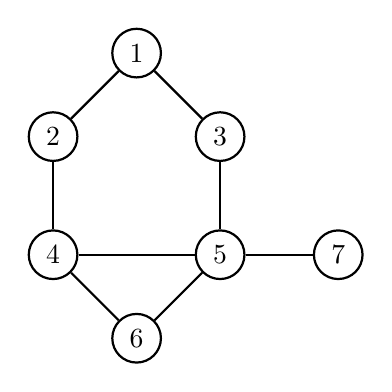
\begin{tikzpicture}[node distance={15mm}, thick, main/.style = {draw, circle}] 
            \node[main] (1) {$1$}; 
            \node[main] (2) [below left of=1] {$2$}; 
            \node[main] (3) [below right of=1] {$3$}; 
            \node[main] (4) [below of=2] {$4$}; 
            \node[main] (5) [below of=3] {$5$};
            \node[main] (6) [below right of=4] {$6$};
            \node[main] (7) [right of=5] {$7$};
            \draw (1) -- (2); 
            \draw (1) -- (3); 
            \draw (2) -- (4);
            \draw (3) -- (5);
            \draw (4) -- (5);
            \draw (4) -- (6);
            \draw (5) -- (6);
            \draw (5) -- (7);
\end{tikzpicture}\newline\newline
\textbf{DFS:} $1 \rightarrow 2 \rightarrow 3 \rightarrow 4 \rightarrow 5 \rightarrow 6 \rightarrow 7$
\begin{itemize}
    \item $L_{0} = \{1\}$
    \item $L_{1} = \{2, 3\}$
    \item $L_{2} = \{4, 5\}$
    \item $L_{3} = \{6, 7\}$
\end{itemize}

\subsection{Correctness}
At the end of BFS($G, s$) we have:
\begin{enumerate}
    \item All the vertices in $C_{s}$ are visited and all the edges are labelled \textit{Discovery Edges} or \textit{Cross Edges}

    \item The set of \textit{Discovery Edges} are a spanning tree $T$ of $C_{s}$ which is called BFS Tree.

    \item $\forall v \in L_{i}$ the path in $T$ from $s$ to $v$ has $i$ edges and every other path from $s$ to $v$ has at least $i$ edges (i.e. $\geq i$ edges)
\end{enumerate}
The proof of the first two properties is the same as for the DFS.\newline\newline
\textbf{Proof of 3:}\newline
Let $P: s = u_{0} \rightarrow u_{1} \rightarrow ... \rightarrow u_{i} = v$ a path from $s$ to $v$, where $u_{j} \in L_{j}$ is \textit{discovered} from the vertex $u_{j - 1} \forall j$. Then, the edge $(u_{j - 1}, u_{j})$ is a \textit{Discovery Edge}. By contradiction, assume assume $\exists$ a path $P': s = z_{0} \rightarrow z_{1} \rightarrow ... \rightarrow z_{t} = v$ with $t < i$. This implies that $ s = z_{0} \in L_{0}$, $z_{1} \in L_{1}$, $z_{2} \in L_{1} \,\, or \,\, L_{2}$, ..., $z_{t} \in L_{1} \,\, or \,\, L_{2} \,\, or \,\,...\,\,L_{t}$. This means that, since $z_{t} = v$, $v \notin L_{i}$, but this is a contradiction.

\subsection{Complexity}
$\forall v \in C_{s}$ there is one iteration of the first \textbf{for} loop and $d(v)$ iterations of the second \textbf{for} loop. Then, the complexity of BFS is:
\[\Theta\left( \sum_{v \in C_{s}} d(v)\right) = \Theta(m_{s})\]

\subsection{Applications}
\begin{itemize}
    \item Same as for DFS in $\Theta(n + m)$ time
    \item Given a graph $G = (V, E)$ and $s,t \in V$ return the \textbf{shortest} path from $s$ to $v$ (if any) \footnote{Shortest path in terms of number of edges between the two nodes}. In order to solve this problem, we can build the path following the same approach as for DFS.
\end{itemize}


\chapter{Lec 04 - Informed Search II}
\section{Recursive Best First Search}
Recursive best-first search (RBFS) is a simple recursive algorithm that attempts to RECURSIVE mimic the operation of standard best-first search, but using only \textbf{linear space}.\newline\newline
Its structure is similar to that of a recursive depth-first search, but
rather than continuing indefinitely down the current path, it uses the \textit{f-limit} variable to keep track of the \textit{f-value} of the best alternative path available from any ancestor of the current node. If the current node exceeds this limit, the recursion unwinds back to the alternative path. As the recursion unwinds, RBFS replaces the \textit{f-value} of each node along the path with a \textbf{backed-up value}, that is, the best \textit{f-value} of its children. In this way, RBFS remembers the \textit{f-value} of the best leaf in the forgotten subtree and can therefore decide whether it’s worth reexpanding the subtree at some later time.
\begin{center}
    \includegraphics[scale=0.8]{images/RBFS-algo.png}
    \includegraphics[]{images/RBFS.png}
\end{center}
Just like A*, RBFS is optimal if the heuristic function $h(n)$ is admissible. Moreover, it has space complexity $O(bd)$ and time complexity which is exponential in the worst case.\newline\newline
The main problem of RBFS (as well as IDA*) is the use of too little memory. In fact, it may happen that the algorithm reexpand forgotten subtrees many times to recreate the best path. Unlike A*, RBFS does not store in the frontier each expanded node, but only the nodes along a single path from the root to a leaf node. 
\newline\newline
In general, the less memory you use, more repetitions you have to do in time. The algorithm MA* (memory-bounded A*) and SMA* (simplified memory-bounded A*) \textbf{fully use all available memory}.

\section{Simplified MA*}
Simplified MA* behaves just like A*, expanding the best node until the memory is full. At this point, it cannot add a new node to the search tree without dropping an old one. SMA* always drops the worst leaf node, that is, the one with the highest \textit{f-value} (last node in the queue). Like RBFS, SMA* then backs up the value of the removed node to its parent. In this way, the ancestor of a forgotten subtree knows the quality of the best path in that subtree. With this information, SMA* regenerates the subtree only when all other paths have been shown to look worse than the path it has forgotten.\newline\newline
What if all the leaf nodes have the same \textit{f-value}? To avoid selecting the same node for deletion and expansion, SMA* expands the newest best leaf and deletes the oldest worst leaf. These coincide when there is only one leaf, but in that case, the current search tree must be a single path from root to leaf that fills all of memory. If the leaf is not a goal node, then even if it is on
an optimal solution path, that solution is \textbf{not reachable with the available memory}.\newline\newline
SMA* properties:
\begin{itemize}
    \item \textbf{complete} only if a solution can be kept in memory
    \item \textbf{optimal} only if any optimal solution is reachable (otherwise it returns the best reachable solution).
\end{itemize}

\section{Heuristic functions}
The performance of heuristic search algorithms depends on the quality of the heuristic function. Let's look, as an example, at heuristics for the 8-puzzle
\begin{center}
    \includegraphics[]{images/8-puzzle.png}
\end{center}
If we want to find the shortest solutions by using A*, we need a heuristic function that never overestimates the number of steps to the goal. There is a long history of such heuristics for the 8-puzzle; here are two commonly used candidates:
\begin{itemize}
    \item $h_1(n) =$ number of misplaced tiles. The start state above would have $h_1(S) = 6$.
    \item $h_2(n) =$ total Manhattan distance, that is, the sum of the distances of the tiles from their goal positions. The state start $S$ qould have $h_2(S) = 4 + 0 + 3 + 3 + 1 + 0 + 2 + 1 = 14$.
\end{itemize}
$h_1$ is faster to compute than $h_2$, however, if $h_2(n) \geq h_1(n)$ for all $n$ (both admissible), then $h_2$ \textbf{dominates} $h_1$. Domination translates directly into efficiency: A* using
$h_2$ will never expand more nodes than $A*$ using $h_1$ (except possibly for some nodes with $f(n) = C^*$). Recall that $A*$ expand all nodes with $f(n) < C^*$ (which is mandatory for any optimal algorithm). This is the same as saying that every node with $h(n) < C^* - g(n)$ will surely be expanded. But because $h_2$ is at least as big as $h_1$ for all nodes, every node that is surely expanded by A* search with $h_2$ will also surely be expanded with $h_1$, and $h_1$ might cause other nodes to be expanded as well. Hence, it is generally better to use a heuristic function with higher value, provided it is consistent and that the computation time for the heuristic is not too long.\newline\newline
Admissible heuristics can be derived from the exact solution cost of
a \textbf{relaxed} version of the problem. A relaxed problem is a problem with fewer restrictions on the actions than the original.\newline\newline
If the rules of the 8-puzzle are relaxed so that a tile can move anywhere, then $h_1(n)$ gives the shortest solution. If the rules are relaxed so that a tile can cove to any adjacent square, then $h_2(n)$ gives the shortest solution.\newline\newline
The key point is that the optimal solution cost of a relaxed problem is no greater than the optimal solution cost of the real problem. Hence, the cost of an optimal solution to a relaxed problem is an \textbf{admissible} heuristic for the original problem.\newline\newline
For example, we can derive a lower bound on the shortest tour for the Travelling Salesman Problem (TSP) using a Minimum Spanning Tree (which can be computed in $O(n^2)$).

\section{Iterative Improvements Algorithms}
If the path to the goal does not matter, we might consider a different class of algorithms, ones that do not worry about paths at all. \textbf{Local search algorithms} operate using a single current node (rather than multiple paths) and generally move only to neighbors of that node. In this case, the \textbf{state space} is the set of \textit{complete} configurations and the task is to find the \textbf{optimal} configuration (e.g. TSP), or to find a configuration satisfying constraints (e.g. timetable).\newline\newline
Local search algorithms have two key advantages: (1) they use very little memory, usually a constant amount, since the paths followed by the search are not retained; and (2) they can often find reasonable solutions in large or infinite (continuous) state spaces for which systematic algorithms are unsuitable.\newline\newline
In addition to finding goals, local search algorithms are useful for solving pure optimization problems, in which the aim is to find the best state according to an \textbf{objective function}.\newline\newline
To understand local search, we find it useful to consider the state-space landscape. A landscape has both “location” (defined by the state) and “elevation” (defined by the value of the heuristic cost function or objective function). If elevation corresponds to cost, then the aim is to find the lowest valley, a \textbf{global minimum}; if elevation corresponds to an objective function, then the aim is to find the highest peak—a global maximum.  Local search algorithms explore this landscape. A complete local search algorithm always finds a goal if one exists; an optimal algorithm always finds a global minimum/maximum.
\begin{center}
    \includegraphics[scale=0.8]{images/state landscape.png}
\end{center}

\subsection{Hill-climbing}
The \textbf{hill-climbing} search algorithm is simply a loop that continually moves in the direction of increasing value, that is, uphill. At each step the current node is replaced by the best neighbor, i.e., the neighbor with the highest \textbf{value} (or lowest heuristic cost if a heuristic is used). It terminates when it reaches a “peak” where no neighbor has a higher value.
\begin{center}
    \includegraphics[]{images/hill-climbing.png}
\end{center}
To illustrate hill climbing, we will use the \textbf{8-queens problem}. Local search algorithms typically use a complete-state formulation, where each state has 8 queens on the board, one per column. The successors of a state are all possible states generated by moving a single queen to another square in the same column (so each state has $8 \times 7 = 56$ successors). The heuristic cost function $h$ is the number of pairs of queens that
are attacking each other, either directly or indirectly. The global minimum of this function is zero, which occurs only at perfect solutions.
\begin{center}
    \includegraphics[scale=0.8]{images/8-queens.png}
\end{center}
Hill climbing often makes rapid progress toward a solution because it is usually quite easy to improve a bad state. Unfortunately, hill climbing often gets stuck for the following reasons:
\begin{itemize}
    \item \textbf{Local maxima:}  a local maximum is a peak that is higher than each of its neighboring states but lower than the global maximum.

    \item \textbf{Ridges:} Ridges result in a sequence of local maxima that is very difficult for greedy algorithms to navigate.

    \item \textbf{Plateaux:} a plateau is a flat area of the state-space landscape. It can be a flat local maximum, from which no uphill exit exists, or a shoulder, from which progress is possible.
\end{itemize}
A possible solution to the \textbf{plateaux} problem is to allow \textbf{sideways move}, i.e, move to a state with same $h$ value, in the hope that the plateau is really a shoulder. In fact, if we are on a flat maxima, an infinite loop will occur. The solution to above problem is to put a limit on the number of consecutive sideways moves allowed.\newline\newline
Many variants of hill climbing have been invented to face the problem of \textbf{local maxima}. \textbf{Stochastic hill climbing} chooses at
random from among the uphill moves; the probability of selection can vary with the steepness of the uphill move. This usually converges more slowly than steepest ascent, but in some state landscapes, it finds better solutions. \textbf{Random-restart hill climbing} conducts a series of hill-climbing searches from randomly generated initial states. It can be proved that if $p$ is the probability to find an optimal solution for a single
search, the expected number of searches needed to find an optimal solution is $1/p$.\newline\newline
Going back to the 8-queens problem, Starting from a randomly generated 8-queens state, \textbf{standard} steepest-ascent hill climbing gets stuck 86\% of the time, solving only 14\% of problem instances.  It works quickly, taking just 4 steps on average when it succeeds and 3 when it gets stuck, not bad for a state space with $8^8 \approx 17$ million states.\newline\newline
Hill-climbing with \textbf{sideways moves} ($\leq 100$ consecutive moves) raises the percentage of problem instances solved to 94\%. On the average it takes around 21 steps to find a solution, otherwise around 64 steps for finding suboptimal solution.\newline\newline
\textbf{Random-restart hill climbing}, for 8-queens instances with no sideways moves allowed ($p \approx 0.14$), needs roughly 7 iterations to find a goal (6 failures and 1 success). The expected number of steps is the cost of one successful iteration plus $(1-p)/p$ times the cost of failure, or roughly 22 steps in all. When we allow sideways moves, the optimal solution is found with probability $p = 0.94$ of times, thus around 1.06 searches to find optimal solution. Total expected number of steps: $63(1  p)/p + 21 = 25.08$.

\chapter{Lec 05 - Prim's \& Kruskal's algorithms}

\section{Efficient Prim's algorithm}
The \textit{standard} implementation of Prim's algorithm has a complexity of $O(m \cdot n)$. For small graph it is an efficient algorithm, but it is not so efficient in very large graphs (e.g. Facebook graph).\newline\newline
In the basic implementation the calculation of a light-edge (i.e. the \textbf{minimum} cross edge with respect to the cut $(S, V \setminus S)$) is done repeatedly. If we are able to speed-up this computation, then the algorithm will be faster. This kind of optimization can be done using a \textbf{heap}. A heap is a data structure which supports the following operations:
\begin{itemize}
    \item \textbf{insert:} add an object to the heap
    \item \textbf{extractMin:} remove the object with the smallest key (highest priority)
    \item \textbf{delete:} given a pointer to an object, remove it.
\end{itemize}
In a heap with $n$ objects, the complexity of these operations is $O(log(n))$\newline\newline
We can redefine the Prim's algorithm exploiting this efficient data structure:
\begin{algorithm}
\caption{Prim}\label{Prim}
    \begin{algorithmic}[1]
    \Procedure{Prim ($G, s$)}{}
        \For{$v \in V$}
            \State Key($v$) $= + \infty$
            \State $\Pi(v) = null$
        \EndFor
        \State Key($s$) = 0
        \State $H = V$
        \While{$H \neq \emptyset$}
            \State $v^{*} = \text{extractMin}(H)$
            \For{$v$ adjacent to $v^{*}$}
                \If{$v \in H$ and $w(v^{*}, v) < \text{Key($v$)}$}
                    \State $\Pi(v) = v^{*}$
                    \State $\text{Key($v$)} = w(v^{*}, v) \quad \text{//Updating the heap}$
                \EndIf
            \EndFor
        \EndWhile
    \EndProcedure
    \end{algorithmic}
\end{algorithm}\newline\newline
$H$ is the heap which contains all the vertices not in the tree. $\Pi(v)$ denotes the parent of $v$ in the tree.\newline\newline %Set A ?
\textbf{Complexity:}
The algorithm performs an initialization, a while loop and a for loop. Let's see the complexity of each of these operations:
\begin{itemize}
    \item \textbf{init:} $O(n)$
    \item \textbf{while:} $n$ iterations
    \item \textbf{extractMin:} $O(log(n))$
\end{itemize}
Total cost of extractMin $\rightarrow O(n\,log(n))$
\begin{itemize}
    \item \textbf{for loop:} executed $O(m)$ times in total:
    \begin{itemize}
        \item $v \in H \rightarrow O(1)$
        \item $\text{Key($v$)} = w(v^{*}, v) \rightarrow O(log(n))$
    \end{itemize}
\end{itemize}
Total cost of for loop $\rightarrow O(m\,log(n))$. \newline\newline
Then, the total complexity of the algorithm is $O(n\,log(n) + m\,log(n))$. Since the graph is connected, it becomes $O(m\,log(n))$.

\section{Kruskal's algorithm}
Kruskal's algorithm is another algorithm for the MST problem which implements the Generic-MST algorithm. In particular:
\begin{itemize}
    \item $A$ is a forest (set of trees)
    \item \textit{safe edge} is a light-edge connecting two distinct components
\end{itemize}
\begin{algorithm}
\caption{Kruskal}\label{kruskal}
    \begin{algorithmic}[1]
    \Procedure{Kruskal ($G$)}{}
        \State $A = \emptyset$
        \State Sort edges of $G$ by weight
        \For{edge $e$ in non-decreasing order}
            \If{$A \cup \{e\}$ is acyclic}
                \State $A = A \cup \{e\}$
            \EndIf
        \EndFor
        \Return $A$
    \EndProcedure
    \end{algorithmic}
\end{algorithm}
Note that:
\begin{itemize}
    \item A source vertex is not needed
    \item We can perform a simple optimization, that is, stop the for loop when $A$ has $n-1$ edges.
\end{itemize}
\textbf{Correctness:} Follows from correctness of Generic-MST.\newline\newline
\textbf{Complexity:}
\begin{itemize}
    \item \textbf{sorting:} $O(m\,log(n))$
    \item \textbf{for loop:} check whether $e = (u,v)$ closes a cycle, which has a complexity of $O(n)$ (DFS implementation). 
\end{itemize}
Then, the total complexity is $O(m \cdot n)$.


\chapter{Lec 06 - Probability}

\section{Probability - terminology}
\begin{itemize}
    \item \textbf{Random variable:} a variable that can take different values randomly

    \item \textbf{Probability distribution:} a description of how likely a random variable x (or a set of random variables) is to take each of its possible states.\newline\newline
    \textbf{Discrete variables:} Probability distribution is described by a \textbf{Probability mass function}
    \begin{itemize}
        \item The domain of $P$ is the set of all possible states of x ($k$ different values).
        
        \item $\forall \, x \in \text{x} \, 0 \leq P(\text{x} = x) \leq 1$
        
        \item $\sum_{x \in \text{x}}P(x) = 1$
    \end{itemize}
    E.g. Uniform distribution $\forall \, x \in \text{x} \, P(\text{x} = x) = \frac{1}{k}$\newline\newline
    \textbf{Continuous variables:} Probability distribution is described by a \textbf{Probability Density Function} (PDF) 
    \begin{itemize}
        \item The domain of $p$ is the set of all possible states of x

        \item $\forall \, x \in \text{x}\, p(x) \geq 0$

        \item $\int p(x) dx = 1$
    \end{itemize}
    E.g. Gaussian distribution

    \item \textbf{Joint probability distribution:} Probability distribution over 2 or more variables $P(\text{x} = x, \text{y} = y)$

    \item \textbf{Gaussian distribution}: The one-dimensional Gaussian with mean $\mu$ and standard deviation $\sigma$ has the following shape:
    \[G(x) = \frac{1}{\sigma \sqrt{2\pi}}e^{-\frac{(x-\mu)^{2}}{2\sigma^{2}}}\]
    \begin{center}
        \includegraphics[]{images/Gaussian.png}
    \end{center}

    \item \textbf{Shannon Entropy (discrete variable):} 
    We can apply information theory to calculate the amount of information there is in an event. This is called \textit{self-information} and can be calculated for a \textbf{discrete} event $x$ as follows:
    \[I(x) = -log\,(P(x))\]
    where $log()$ is the base-2 logarithm and $P(x)$ is the probability of the event $x$ \footnote{other bases can be used, $e$ for example}.
    \newline\newline
    The choice of the base-2 logarithm means that the units of the information measure is in bits (binary digits). This can be directly interpreted as the number of bits required to represent an event. If the probability that an event occurs is $0.5$, we need 1 bit two represent it ($0$ fail, $1$ success); if the event occurs with probability $0.125$, we need $3$ bits to represent it (remember $y = log_a\,(x) \iff x = a^y$).
    \newline\newline
    The Shannon entropy of a \textbf{distribution} is the \textbf{expected} amount of information in an event drawn from that distribution:
    \[H(\text{x}) = - E_{x \sim P(\text{x})}[log(P(x))] = -\sum_i P(x_i) log\,P(x_i)\]
    It provides a lower bound on the number of bits needed \textbf{on average} to encode a symbol drawn from the distribution.\newline\newline
    Distributions that are nearly deterministic (where the outcome is nearly certain) have low entropy; distributions that are closer to uniform have high entropy.
    

    \item \textbf{Kullback-Leibler divergence and Cross Entropy:} Let's consider two probability distributions $P(x)$ and $Q(x)$. How can we measure how different they are?
    \begin{itemize}
        \item Kullback-Leiber divergence:
        \[D_{KL}(P \,||\, Q) = E_{x \sim P}\left[ log\frac{P(x)}{Q(x)} \right] = E_{x \sim P}[ log\, P(x) - log\, Q(x)] = \sum_i P(x_i) log\, \left(\frac{P(x_i)}{Q(x_i)}\right)\]
        It is not a true distance because it is not symmetric:
        \[D_{KL}(P \, ||\, Q) \neq D_{KL}(Q \, ||\, P)\]
        It is the measure of information lost when $Q$ is used to approximate $P$.


        \item Cross Entropy:
        \[H(P, Q) = H(P) + D_{KL}(P\, ||\, Q) = -E_{x \sim P}[log\, Q(x)]\]
        where $H(P)$ is the entropy of $P$. Note that minimizing the Cross Entropy of $P$ with respect to $Q$ is equivalent to minimize KL divergence between $P$ and $Q$. (if $P$ is given, $H(P)$ and $E_{x \sim P}[log\, P(x)]$ are constants). If $P$ is a fixed distribution minimize KL divergence or minimize CE is the same, but CE is easier to compute.
    \end{itemize}

    \item \textbf{Maximum likelihood estimation:} Is a principled way to derive estimators (models). Consider $n$ examples $Tr = \{\textbf{x}^{1}, ..., \textbf{x}^{n}\}$ drawn i.i.d. from $p_{data}$ (which is not known in advance). With machine learning we want to estimate this probability $p_{data}$ with some models that depend on a set of parameters $\theta$.\newline\newline
    Let's consider a family of parametric probability distributions (models) $p_{model}(\textbf{x}; \theta)$. It maps a point $\textbf{x}$ to a real number, estimating $p_{data} (\textbf{x})$. How can we find $\theta$ in such a way that $p_{model}$ and $p_{data}$ are as close as possible ? A possible formalization of this problem is given by the Maximum Likelihood estimation for $\theta$:
    \[\theta_{ML} = argmax_{\theta}\, p_{model}(Tr; \theta) = argmax_{\theta}\prod_{i = 1}^{n}p_{model}(\textbf{x}^{i}; \theta)\]
    Basically, we choose the probability distribution which is most likely to have produced our data. Note that we are assuming that all the examples are \textbf{independent} each other ($P(x, y) = P(x)P(y)$).
\end{itemize}

\section{Maximum likelihood}
Maximum likelihood (ML) is a special case of \textbf{maximum a posteriori estimation (MAP)}.
\[h_{MAP} = argmax_{h \in H}P(h|D)\]
\[= argmax_{h \in H}\frac{P(D|h)P(h)}{P(D)}\]
where:
\begin{itemize}
    \item $P(h):$ a priori probability of the hypothesis $h$
    \item $P(D):$ a priori probability of training data. It is the probability to observe exactly this training set when we don't know anything about the hypothesis.
    \item $P(h|D):$ probability of $h$ given $D$. It is the probability that $h$ is the hypothesis that generates data $D$.
    \item $P(D|h):$ probability if $D$ given $h$. Given a hypothesis $h$, it is the probability of data $D$ to be generated by $h$.
\end{itemize}
Since $P(D)$ does not depend on $h$, we can consider it as a constant and remove it from the equation.
\[= argmax_{h \in H}P(D|h)P(h)\]
If we assume uniform probabilities on the hypotheses, that is $P(h_{i}) = P(h_{j})$, we can choose the so called \textbf{maximum likelihood hypothesis} $h_{ML}:$
\[h_{ML} = argmax_{h \in H}P(D|h)\]
MAP and maximum likelihood approach make predictions using a single point estimate of $\theta$. The Bayesian approach is to make predictions using a full probability distribution over $\theta$. For example, given a new instance $\textbf{x}$, which is the most likely \textbf{classification}? The classification given by the most likely hypothesis $h_{MAP}$ is not necessarily the most likely classification. For example, given the following three possible hypothesis:
 \[P(h_{1} | D) = 0.4 \quad P(h_{2} | D) = 0.3 \quad P(h_{3} | D) = 0.3\]
 We want to classify a new instance $\textbf{x}$:
 \[h_{1}(\textbf{x}) = + \quad h_{2}(\textbf{x}) = - \quad h_{1}(\textbf{x}) = -\]
 The most likely hypothesis $h_{1}$ classifies $\textbf{x}$ with the label (+), but the most likely classification is (-). This is because the optimal (Bayes) classification of a certain instance is the class $v_{j} \in V$ which maximizes the following probability:
 \[argmax_{v_{j} \in V} = \sum_{h_{i} \in H}P(v_{j} | h_{i})P(h_{i} | D)\]
 where $V$ is the set of possible labels.\newline\newline
 However, in real-world problems having the probabilities $P(h_{i} | D)$ is almost impossible. Therefore, we usually make the assumption of considering the classification made by $h_{map}$ as most probable.

 \subsection{Maximum likelihood estimation}
 As we said before, the maximum likelihood estimation is defined as follows:
 \[\theta_{ML} = argmax_{\theta}\, p_{model}(Tr; \theta) = argmax_{\theta}\prod_{i = 1}^{n}p_{model}(\textbf{x}^{i}; \theta)\]
 However, computing the product of many probability is unstable. Therefore, we can apply the $log$ and the $argmax$ does not change (log-likelihood).
 \[\theta_{ML} = log(argmax_{\theta}\prod_{i=1}^{n}p_{model}(\textbf{x}^{(i)}; \theta))\]
 \[= argmax_{\theta}\sum_{i = 1}^{n}log\, p_{model}(\textbf{x}^{(i)}, \theta)\]
 We can equivalently divide by $n$ to express maximum likelihood as an expectation over training data:
 \[\theta_{ML} = argmax_{\theta}E_{x \sim \hat{p}_{data}}[log \, p_{model}(x; \theta)]\]
where $\hat{p}_{data}$ is an empirical discrete distribution that we get over the examples in the training set. This implies that maximum likelihood minimizes the dissimilarity between $\hat{p}_{data}$ and $p_{model}$, measured by the KL divergence. It also corresponds to minimize the \textbf{cross-entropy} between the two distributions.

\subsection{Conditional log likelihood}
We can use maximum likelihood to estimate a \textbf{conditional} probability $P(\textbf{y} | \textbf{x}; \theta)$ to predict $\textbf{y}$ given $\textbf{x}$ (supervised learning).
\[\theta_{ML} = argmax_{\theta} P(\textbf{Y} | \textbf{X}; \theta)\]
If input examples are i.i.d.
\[\theta_{ML} = argmax_{\theta}\sum_{i=1}^{n}log\, P(\textbf{y}^{(i)} | \textbf{x}^{(i)}; \theta)\]
Consider any real-valued target function $f$ and learning examples $\langle 
 \textbf{x}_{i}, d_{i}\rangle$ where $d_{i}$ has some noise:
 \begin{itemize}
     \item $d_{i} = f(\textbf{x}_{i}) + e_{i}$
     \item $e_{i}$ is a random variable (noise) extracted independently, for each $\textbf{x}_{i}$, according to a Gaussian distribution with mean 0.
 \end{itemize}
 It can be shown that the maximum likelihood hypothesis is the one that minimizes the mean squared error:
 \[\theta_{ML} = argmin_{\theta} \sum_{i=0}^{m}(d_{i} - \hat{y}_{i})^{2}\]
maximizing the log-likelihood with respect to $\theta$ yields the same estimate of the parameters $\theta$ as does minimizing the mean squared error.

\chapter{Lec 07 - Neural Networks I}

\section{Neural Networks}
An artificial neuron is a unit that computes a non-linear function over the inputs. Its output depends on the input and on the set of \textbf{weights}. These weights have to be learned.\newline\newline
An \textbf{Artificial Neural Network} is a system consisting of interconnected units that compute nonlinear (numerical) functions. Adjustable weights are associated with connections among units.\newline\newline
Deep Feed Forward Neural Networks, also called multi-layer perceptrons (MLP), approximate a function $f^{*}$ that maps an input $x$ to a category $y$. The MLP defines a mapping $\hat{y} = f(x;\theta)$ where $\theta$ is the set of parameters. They are typically represented as a composition of many different functions $f(x) = f^{(3)}(f^{(2)}(f^{(1)}(x)))$. The intermediate layers are called \textbf{hidden layers}, while the final layer is called \textbf{output layer}.\newline\newline
Multiple layers of cascaded units makes a Neural Network able to implement complex non linear functions. The non linearity of the model is given by the activation functions. In fact, without them (linear activation) the result of the model, even if it’s very complex, would still be linear.\newline\newline
\textbf{Example:}\newline
Let's try to define a linear model that predicts the XOR function.
\[Tr = \{ ([0,0], 0), ([0, 1], 1), ([1,0],1), ([1,1], 0)\} \quad f(\textbf{x};\textbf{w};b) = \textbf{x}\textbf{w}^{T} + b\]
The XOR function \textbf{cannot} be learned by any linear classifier. In order to solve this problem, we can define a two-layers Neural Network with the addition of the ReLU activation function $ReLU(y) = max(0, y)$. The networks becomes:
\[f(\textbf{x}; \textbf{W}, \textbf{c}, \textbf{w}, b) = \textbf{w}^{T} \, max(0, \textbf{W}\textbf{x}^{T} + \textbf{c}) + b\]
the following parameters values provide a solution to the XOR problem:
\[
    \textbf{W} =
    \begin{bmatrix}
        1 & 1\\
        1 & 1
    \end{bmatrix},
    \,\,
    \textbf{c} = 
    \begin{bmatrix}
        0 \\
        -1
    \end{bmatrix},
    \,\,
    \textbf{w} = 
    \begin{bmatrix}
        1 \\
        -2
    \end{bmatrix},
    \,\,
    b = 0
\]
Note that the first hidden layer has two nodes.\newline\newline
The most common activation functions are the following:
\begin{center}
    \includegraphics[scale = 0.6]{images/Activation Functions.png}
\end{center}
In general, the goal is to have a more complex decision surface. We can achieve this goal by using non-linear activation functions and stacking several hidden layers. In the XOR example above, the initial points are mapped by the first hidden layer into a new space where they are linearly separable. Thanks to this, the output linear layer is able to classify the points correctly.

\section{Learning in a Neural Network}
In general, the problem of how to update the weights of a model in order to minimize the committed error is called \textbf{credit assignment problem}. A possible solution is to make a single neuron \textbf{derivable} and exploit gradient descent technique to learn the \textit{right} weights. In order to make a neuron derivable, its activation function must be derivable.\newline\newline
Linear models (e.g. SVM) are formulated as \textbf{convex models}. However, the non-linearity in neural networks makes the problem \textbf{non-convex}. It means that there is no guarantee of achieving the global optimum. Furthermore, the way in which the weight of a NN are initialized has a strong impact on the solution that the model will find.

\section{Cost Function}
A important aspect of the design of a deep neural network is the choice of the cost function. In most cases, the model defines a distribution $p(\textbf{y} | \textbf{x}; \theta)$ and the cost function is the cross-entropy between training labels and network predictions (negative log-likelihood):
\[J(\theta) = - E_{(x,y) \sim \hat{p}_{data}}log\, p_{model}(\textbf{y}|\textbf{x})\]
The specific form of the cost function changes from model to model. The output representation $\textbf{h} = f(\textbf{x};\theta)$ determines the form of the cross-entropy function.
\begin{itemize}
    \item \textbf{Linear Regression:} If we assume that the target values are distributed according to a Gaussian distribution $G$, we can think our output layer as to produce the mean of $G$.
    \[\hat{\textbf{y}} = \textbf{W}^{T}\textbf{h} + \textbf{b}\]
    \[G(\textbf{y};\hat{\textbf{y}}; \textbf{I})\]
    As we already seen, in this case maximizing the likelihood corresponds to minimize the mean squared error.
    \[J(\theta) = \frac{1}{2}E_{p \sim \hat{p}_{data}}(y - f(\textbf{x}; \theta))^{2} + constant\]
    Basically, this is a motivation of why the mean squared error cost function is suitable for linear regression.

    \item \textbf{Binary classification:} In this case we assume that our targets are distributed according to a Bernoulli distribution. This distribution depends on a single parameter $\phi \in [0, 1]$:
    \begin{itemize}
        \item $P(\text{x} = 1) = \phi$
        \item $P(\text{x} = 0) = 1 - \phi$
    \end{itemize}
    In general:
    \[P(\text{x} = x) = \phi^{x}(1 - \phi)^{1-x}\]
    The NN just needs to predict $P(\text{y} = 1 | \textbf{x})$. Therefore, we want to force this number to lie in $[0, 1]$. For example, we can use the following function:
    \[P(\text{y} = 1|\textbf{x}) = max(0, min(1, \textbf{w}^{T}\textbf{h} + b))\]
    However, this is not a good choice for gradient descent. In fact, if the output is outside $[0, 1]$ the function is not derivable and the gradient will always be 0. We want to ensure that there is always some gradient when the model is wrong. An alternative way to force the output to lie in $[0, 1]$ is to use an \textbf{output} linear layer with a \textbf{sigmoid activation function}.
    \[\hat{y} = \sigma(\textbf{w}^{T}\textbf{h} + b)\]
    where $\sigma$ is a Sigmoid or Logistic function:
    \[\sigma(x) = \frac{1}{1 + e^{-x}}\]
    \begin{center}
        \includegraphics[scale = 0.5]{images/sigmoid.png}
    \end{center}
    An output unit is composed of two components:
    \begin{itemize}
        \item $z = \textbf{w}^{T}\textbf{h} + b$
        \item $\sigma(\cdot)$: the activation function to \textbf{convert $z$ into a probability} (in order to apply maximum likelihood optimization).
    \end{itemize}
    How can we define a probability distribution over $y$ using the value $z$ ? The sigmoid can be motivated by constructing an unnormalized probability distribution $\hat{P}(y)$, which does not sum to 1. We assume that the unnormalized probabilities are linear in $y$ and $z$.
    \[log\, \hat{P}(y) = yz \quad i.e. \,\, log\, \hat{P}(y = 1) = z, \,\, log\, \hat{P}(y = 0) = 0\]
    We can exponentiate to obtain the unnormalized probabilities:
    \[\hat{P}(y) = e^{yz}\]
    Then, we normalize to obtain a proper probablity:
    \[P(y) = \frac{e^{yz}}{\sum_{y'=0}^{1} e^{y'z}} = \sigma((2y - 1)z)\]
    where:
    \begin{itemize}
        \item $P(y = 1) = \frac{1}{1 + e^{-z}}$
        \item $P(y = 0) = \frac{1}{1 + e^{z}}$
    \end{itemize}
    As we already seen, the cost function used with maximum likelihood is the negative-log likelihood. Therefore, the loss function for maximum likelihood learning of a Bernoulli parametrized by a sigmoid is:
    \[J(\theta) = -log\, P(y|\textbf{x}) = -log\,\sigma((2y - 1)z) = \zeta((1 - 2y)z)\]
    where $\zeta(x) = log(1 - exp(x))$ is called \textbf{softplus} function.\newline\newline
    This approach to predicting the probabilities in log-space is natural to use with maximum likelihood learning. The log in the cost function undoes the exp of the sigmoid. Without this effect, the saturation of the sigmoid could prevent gradient- based learning from making good progress.\newline\newline
    The saturation (i.e. when the gradient is very small) occurs when $y = 1$ and $z$ is very positive or $y = 0$ and $z$ is very negative, that is, when the model has the right answer.\newline\newline
    With other cost functions, such as MSE, we'll be able to find a solution but it would \textbf{not} be the maximum-likelihood solution.

    \item \textbf{Multi-class classification:} In this case the output has to be a probability distribution over a discrete variable with $n$ possible values. We have to generate a vector $\hat{\textbf{y}}= [\hat{y}_0, \hat{y}_1, ..., \hat{y}_{n-1}]$ where:
    \begin{itemize}
        \item $\hat{y}_i = P(y = i | \textbf{x})$
        \item $\forall i,\,\, 0 \leq \hat{y}_i \leq 1$
        \item $\sum_i \hat{y}_i = 1$
    \end{itemize}
    We can use the same approach for the Bernoulli distribution generalized to the \textbf{Multinoulli distribution}:
    \[\textbf{z} = \textbf{W}^{T}\textbf{h} + \textbf{b} \quad \text{where}\,\, z_i = log\, \hat{P}(y = i | x)\]
    In order to represent the probability distribution over $n$ different classes, we can use the \textbf{Softmax} function, which is a generalization of sigmoid.
    \[softmax(\textbf{z})_i = \frac{e^{z_i}}{\sum_j^n e^{z_j}}\]
    By applying the log-likelihood, the cost function is:
    \[log\, softmax(\textbf{z})_i = z_i - log \, \sum_j e^{z_j}\]
    $z_i$ pushes the correct labels up and $log \, \sum_j e^{z_j}$ pushes the uncorrect labels down. When we perform the prediction, we'll choose the argmax of $\hat{\textbf{y}}$.
\end{itemize}

\subsection{Output functions in general}
Linear, sigmoid and softmax output units are the most common, but NN can generalize to almost any kind of output layer.\newline\newline
Maximum likelihood provides a guide to design almost any output layer.
\begin{enumerate}
    \item We define a conditional distribution $p(\textbf{y}|\textbf{x}; \theta)$
    \item As cost function, maximum likelihood suggest to use $-log\, p(\textbf{y}|\textbf{x}; \theta)$
\end{enumerate}
We can think of the NN as $f(\textbf{x}; \theta) = \omega$ where $\omega$ are the parameters of a distribution over $\textbf{y}$ and the cost function is $-log\, p(\textbf{y};\omega(\textbf{x}))$

\section{Hidden units}
An hidden unit can be described as accepting an input $x$, computing $z = W^{T}x + b$, and applying an element-wise nonlinear function $g(z)$. The design of hidden units does not have many definitive guiding theoretical principle. What we can do is to evaluate hidden units performance on a validation set. To select the most suitable activation function we can rely on some basic intuitions motivating each type of hidden unit.

\subsection{Hidden units: ReLU}
An hidden unit with ReLU activation function is defined as follows:
\[g(z) = max(0, z) \quad z = f(\textbf{W}^{T}\textbf{x} + \textbf{b})\]
Such hidden units are similar to linear units and therefore easier to optimize. However, ReLU units do not learn via gradient-based methods on examples for which their activation is zero. In order to solve this problem, generalizations of ReLU have been defined (e.g. leakyReLU) $g(z, \alpha)_i = max(0, z_i) + \alpha_i \, min(0, z_i)$.

\subsection{Hidden units: Tanh and sigmoid}
Other common activation functions are Tanh and sigmoid:
\begin{itemize}
    \item Logistic sigmoid: $g(z) = \sigma(z)$
    \item Hyperbolic Tangent: $g(z) = tanh(z) = 2\sigma(2z) - 1$
\end{itemize}
Actually, these two functions are not a very good choice for the hidden layers since they saturate across most of their domain. In particular, they saturate to high value when $z$ is very positive, and to low value when $z$ is very negative. This is good for output units, as we seen before, but not for hidden units, because in hidden layers we just want to keep learning without necessarily having a value between 0 and 1. Tanh typically performs better than the logistic sigmoid.\newline\newline
In general, many differentiable functions are reasonable (e.g. $cos(x)$), but they show no significant advantage over common ones.

\section{Architecture}
The architecture of a NN is its overall structure. Neural networks are generally organised in layers where each layer is a function of the preceding one:
\[\textbf{h}^{(1)} = g^{(1)}(\textbf{W}^{(1)T}\textbf{x} + \textbf{b}^{(1)})\]
\[\textbf{h}^{(i)} = g^{(i)}(\textbf{W}^{(i)T}\textbf{h}^{(i - 1)} + \textbf{b}^{(i)})\]
The main architectural considerations are:
\begin{itemize}
    \item The depth of the network
    \item The width of each layer
\end{itemize}
Deeper networks tend to generalize better, but they are harder to train.\newline\newline
All these hyper-parameters should be validated on a validation set.\newline\newline
\textbf{Universal approximation Theorem}\newline\newline
Given a feed-forward NN with just one hiddel layer, any continuous function $f:\mathbb{R}^{n} \rightarrow \mathbb{R}$ and an arbitrarily small $\epsilon > 0$, then, for a large class of activation functions, there always exists an integer $M$ such that the function $g: \mathbb{R}^{n} \rightarrow \mathbb{R}$ computed by the net using at least $M$ hidden units approximates the function $f$ with tolerance $\epsilon$, that is:
\[max_{x \in \Omega}|f(\textbf{x}) - g(\textbf{x})| < \epsilon\]
Note that the theorem attests the existence of a NN with $M$ hidden units that approximates any continuous function with the desired tolerance, but it says nothing about how $M$ can be computed and how large this network would be. Furthermore, we are not guaranteed that the training algorithm will be able to learn it (the optimization algorithm may not be able to find the value of the parameters that corresponds to the desired function).\newline\newline
Using deeper models can reduce the number of units required to represent the desired function. Furthermore, greater depth does seem to result (empirically) in better generalization for a wide variety of tasks.\newline\newline
Many neural networks architectures have been developed for specific tasks, e.g. Convolutional Neural Networks (CNN) or Recurrent Neural Network (RNN). In general, the layers need to be connected in a chain:
\begin{itemize}
    \item Skip connections: Make it easier for the gradient to flow from output layers to layers nearer the input.

    \item Sparse connections: Each unit in a layer is connected to only a small subset of units in the next layer.
\end{itemize}

\chapter{Lec 08 - General SSSP Problem}

\section{General SSSP Problem}
In the general formulation of the SSSP problem, the graphs can have edges with negative weights. With negative weights we must be careful about what we mean by shortest path. Let's consider the following graph:

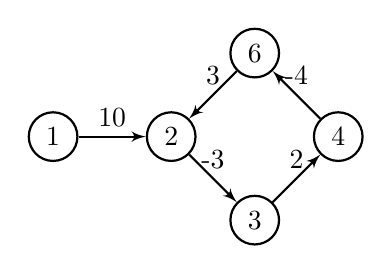
\begin{tikzpicture}[node distance={15mm}, thick, main/.style = {draw, circle}, edge/.style = {->,> = latex'}]
            \node[main] (1) {$1$}; 
            \node[main] (2) [right of=1] {$2$}; 
            \node[main] (3) [below right of=2] {$3$}; 
            \node[main] (4) [above right of=3] {$4$};
            \node[main] (6) [above left of=4] {$6$};

            \draw[edge] (1) -- node[above] {10} (2) ;
            \draw[edge] (2) -- node[above] {-3} (3);
            \draw[edge] (3) -- node[above] {2} (4);
            \draw[edge] (4) -- node[above] {-4} (6);
            \draw[edge] (6) -- node[above] {3} (2);
             
\end{tikzpicture}\newline\newline
This graph contains a \textbf{negative weights cycle}. Let's say that we want to compute the shortest path from $1$ to $2$. If we run Dijkstra algorithm, it will get stucked in the cycle forever. Basically $dist(1, 2) = -\infty$.\newline\newline
Therefore, we need to compute the shortest cycle-free/simple paths. Now the problem is well defined, but it is NP-Hard (problem for which we don't have any polynomial time algorithm).\newline\newline
So let's redefine the SSSP problem in a revised version:
\begin{itemize}
    \item \textbf{input:} A directed weighted graph $G = (V, E)$ and a source vertex $s \in V$.

    \item \textbf{output:} One of the following:
    \begin{enumerate}
        \item $dist(s, v) \,\, \forall v \in V$

        \item A declaration that $G$ contains a negative cycle.
    \end{enumerate}
\end{itemize}
Note that a shortest path \textbf{cannot} contain a cycle, except for 0-weight cycles, but in that case we can just remove all of them.\newline\newline
What needs to be changed in Dijkstra's algorithm in order to make it able to deal with negative-weights edges?\newline\newline
\textbf{Intuition:}\newline\newline
The problem in Dijkstra's algorithm is that it never updates its decisions. $len(v)$ should be an \textbf{estimated distance} and it needs to be updated for every vertex ($n-1$ times because this is the maximum number of edges in a simple path between any two vertices).

\subsection{Bellman-Ford algorithm}
\begin{itemize}
    \item \textbf{input:} A directed graph $G$ with edge weights $w: E \rightarrow \mathbb{R}$, and a source vertex $s \in V$. 
    
    \item \textbf{output:} Either $dist(s, v)$ or a declaration that $G$ contains a negative cycle.

\end{itemize}

\begin{algorithm}
\caption{Bellman-Ford}\label{Bellman-Ford}
    \begin{algorithmic}[1]
    \Procedure{Bellman-Ford ($G, s$)}{}
        \State $len(s) = 0$
        \State $len(v) = \infty \,\, \forall v \neq s$
        \For{$n - 1$ iterations}
            \For{edge $(u, v) \in E$}
                \State $len(v) = min(len(v), len(u) + w(u, v))$
            \EndFor
        \EndFor

        \For{edge $(u, v) \in E$}
            \If{$len(v) > len(u) + w(u, v)$}
                \Return \textit{G contains a negative cycle}
            \EndIf
        \EndFor
    \EndProcedure
    \end{algorithmic}
\end{algorithm}
\textbf{Complexity:} $O(m \cdot n)$.\newline\newline
\textbf{Example:}\newline\newline
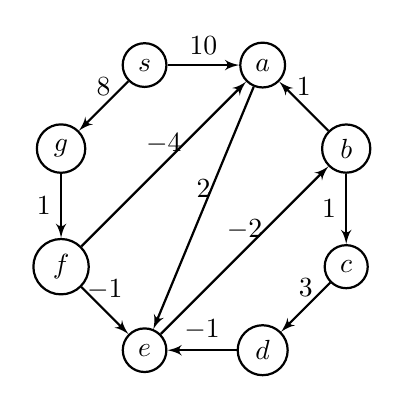
\begin{tikzpicture}[node distance={15mm}, thick, main/.style = {draw, circle}, edge/.style = {->,> = latex'}]
            \node[main] (s) {$s$}; 
            \node[main] (a) [right of=s] {$a$}; 
            \node[main] (b) [below right of=a] {$b$}; 
            \node[main] (c) [below of=b] {$c$};
            \node[main] (d) [below left of=c] {$d$};
            \node[main] (e) [left of=d] {$e$};
            \node[main] (f) [above left of=e] {$f$};
            \node[main] (g) [below left of=s] {$g$};

            \draw[edge] (s) -- node[above] {10} (a) ;
            \draw[edge] (s) -- node[above] {8} (g);
            \draw[edge] (g) -- node[left] {1} (f);
            \draw[edge] (f) -- node[above] {$-4$} (a);
            \draw[edge] (f) -- node[above] {$-1$} (e);
            \draw[edge] (e) -- node[above] {$-2$} (b);
            \draw[edge] (b) -- node[left] {$1$} (c);
            \draw[edge] (c) -- node[above] {$3$} (d);
            \draw[edge] (d) -- node[above] {$-1$} (e);
            \draw[edge] (b) -- node[above] {$1$} (a);
            \draw[edge] (a) -- node[above] {$2$} (e);
\end{tikzpicture}
\vspace{5pt}
\begin{center}
    \begin{tabular}{c| c c c c c c c c|c}
        & 0 & 1 & 2 & 3 & 4 & 5 & 6 & 7 & last\\
        \hline\hline
         $s$ & 0 & 0 & 0 & 0 & 0 & 0 & 0 & 0 & 0 \\
         $a$ & $\infty$ & 10 & 10 & 5 & 5 & 5 & 5 & 5 & 5\\
         $b$ & $\infty$ & $\infty$ & $\infty$ & 10 & 6 & 5 & 5 & 5 & 5\\
         $c$ & $\infty$ & $\infty$ & $\infty$ & $\infty$ & 11 & 7 & 6 & 6 & 6\\
         $d$ & $\infty$ & $\infty$ & $\infty$ & $\infty$ & $\infty$ & 14 & 10 & 9 & 9\\
         $e$ & $\infty$ & $\infty$ & 12 & 8 & 7 & 7 & 7 & 7 & 7\\
         $f$ & $\infty$ & $\infty$ & 9 & 9 & 9 & 9 & 9 & 9 & 9\\
         $g$ & $\infty$ & 8 & 8 & 8 & 8 & 8 & 8 & 8 & 8\\
\end{tabular}
\end{center}
\textbf{Correctness of the algorithm:}\newline\newline
Let $len(i, v)$ be the length of a shortest path from $s$ to $v$ that contains at most $i$ edges. Since the shortest path from $s$ to $v$ contains at most $n - 1$ edges, it's sufficient to prove that after $i$ iterations $len(v) \leq len(i, v)$.\newline\newline
We'll prove it by induction on $i$:
\begin{itemize}
    \item \textbf{Base case:} $i = 0$
    \[len(s) = 0 \leq len(0, s) = 0\]
    \[len(v \neq s) = +\infty = len(0, v \neq s)\]

    \item \textbf{Inductive hypothesis:} $len(v) \leq len(k, v) \,\, \forall \, 1 \leq k \leq i$
\end{itemize}
Take $i \geq 1$ and take a shortest path from $s$ to $v$ with at most $i$ edges. Let $(u, v)$ be the last edge of this path. Then:
\[len(i, v) = len(i - 1, u) + w(u, v)\]
By inductive hypothesis, $len(u) \leq len(i - 1, u)$. In the $i$-th iteration we update $len(v)$ as follows:
\[len(v) = min(len(v), len(u) + w(u, v))\]
\[len(u) + w(u, v) \leq len(i - 1, u) + w(u, v) = len(i, v)\]
Therefore, $len(v) \leq len(i, v)$.


\chapter{Lec 09 - Logical Agents II}
\section{Propositional Theorem Proving}
So far, we have shown how to determine entailment by model checking: enumerating models and showing that the sentence must hold in all models. In this section, we show how entailment can be done by \textbf{theorem proving}, that is, applying rules of \textbf{inference} directly to the sentences in our knowledge base to construct a proof of the desired  sentence without consulting models. 
\newline\newline
Inference rules can be applied to derive a \textbf{proof}, a chain of conclusions that leads to the desired goal. The best-known rule is called \textbf{Modus Ponens}.
\begin{center}
    \includegraphics[]{images/modus-ponens.png}
\end{center}
The notation means that, whenever any sentences of the form $\alpha \Rightarrow \beta$ and $\alpha$ are given, then the sentence $\beta$ can be inferred. For example, if $(WumpusAhead \land WumpusAlive) \Rightarrow Shoot$ and $(WumpusAhead \land WumpusAlive)$ are given, then $Shoot$ can be inferred. These techniques typically require translation of sentences into a \textbf{normal form}.
\newline\newline
Some real-world knowledge bases satisfy certain restrictions on the form of sentences they contain, which enables them to be represented with a restricted form which enables more efficient inference algorithms. One such restricted form is the \textbf{Horn form}, which is a conjunction of Horn clauses. A Horn clause is defined as follows:
\begin{itemize}
    \item proposition symbol; or
    \item (conjunction of symbols) $\Rightarrow$ symbol.
    \[C \land (B \Rightarrow A) \land (C \land B \Rightarrow A)\]
\end{itemize}
In Horn form, the premise is called the \textbf{body} and the conclusion is called the \textbf{head}. A sentence consisting of a single positive literal, such as $P_{1,1}$, is called a \textbf{fact} ($True \Rightarrow P_{1,1}$).\newline\newline
Knowledge bases containing only Horn clauses are interesting for the following reasons:
\begin{itemize}
    \item  Inference with Horn clauses can be done through the forward-chaining and backwardchaining algorithms, which we explain next. Both of these algorithms are natural, in that the inference steps are obvious and easy for humans to follow.

    \item  Deciding entailment with Horn clauses can be done in time that is linear in the size of the knowledge base.
\end{itemize}

\section{Forward and Backward Chaining}
The \textbf{forward-chaining} algorithm  determines if a single proposition symbol $q$, the query, is entailed by a knowledge base of Horn clauses. It begins from known facts in the knowledge base. If all the premises of an implication are known, then its conclusion is added to the set of known facts. For example, if $L_{1,1}$ and $Breeze$ are known and $(L_{1,1} \land Breeze) \Rightarrow B_{1,1}$ is in the knowledge base, then $B_{1,1}$ can be added. This process continues until the query $q$ is added or until no further inferences can be made.
\begin{center}
    \includegraphics[]{images/forward chaining.png}
    \includegraphics[]{images/graph.png}
\end{center}
The best way to understand the algorithm is through an example showed in the figure above. It shows a simple knowledge base of Horn clauses with $A$ and $B$ as known facts represented as an AND-OR graph. In AND–OR graphs, multiple links joined by an arc indicate a conjunction, that is, every link must be proved. While multiple links without an arc indicate a disjunction, any link can be proved.
\begin{center}
    \includegraphics[]{images/frwd exec.png}
\end{center}
Forward chaining is \textbf{sound}: every inference is essentially an application of Modus Ponens. Forward chaining is also \textbf{complete}: every entailed atomic sentence will be derived.\newline\newline
The easiest way to see this is to consider the final state of the \textit{inferred} table (after the algorithm reaches a \textbf{fixed point} where no new inferences are possible). The table contains \textit{true} for each symbol inferred during the process, and \textit{false} for all other symbols. We can view the table as a logical model; moreover, every Horn clause in the original KB is true in this model. To see this, assume the opposite, namely that some clause $a_1\land ...\land a_k \Rightarrow b$ is \textit{false} in the model. Then $a_1\land ...\land a_k$ must be \textit{true} in the model and $b$ must be \textit{false} in the model. But this contradicts our assumption that the algorithm has reached a fixed point. We can conclude, therefore, that the set of atomic sentences inferred at the fixed point defines model of the original KB. Furthermore, any atomic sentence $q$ that is entailed by the KB must be true in all its models and in this model in particular. Hence, every entailed atomic sentence $q$ must be inferred by the algorithm.\newline\newline
The \textbf{backward-chaining} algorithm, as its name suggests, works backward from the query.  If the query $q$ is known to be true, then no work is needed. Otherwise, the algorithm finds those implications in the knowledge base whose conclusion is $q$.  If all the premises of
one of those implications can be proved true (by backward chaining), then $q$ is true.
\begin{center}
    \includegraphics[scale=0.8]{images/bkwrd exec.png}
\end{center}
Forward chaining is an example of the general concept of \textbf{data-driven} reasoning, that is, reasoning in which the focus of attention starts with the known data. However, it may do lots of work that is irrelevant to the goal.\newline\newline
Backward chaining is a form of \textbf{goal-directed} reasoning. It is appropriate for problem solving and for answering specific questions such as “What shall I do now?” and “Where are my keys?" Often, the cost of backward chaining is much less than linear in the size of the knowledge base, because the process touches only relevant facts.

\section{Resolution}
The current section introduces a single inference rule, \textbf{resolution}, that yields a complete inference algorithm when coupled with any complete search algorithm. The resolution rule applies only to disjunctions of literals (clauses), so it would seem
to be relevant only to knowledge bases and queries consisting of clauses. How, then, can it lead to a complete inference procedure for all of propositional logic?  The answer is that every sentence of propositional logic is logically equivalent to a \textbf{conjunction of clauses}. A sentence expressed as a conjunction of clauses is said to be in \textbf{conjunctive normal form} or \textbf{CNF}.\newline\newline
The resolution rule is the following:
\begin{center}
    \includegraphics[]{images/resolution.png}
\end{center}
where $l_i$ and $m_j$ are complementary literals. This says that resolution takes two clauses and produces a new clause containing all the literals of the two original clauses except the two complementary literals. For example:
\begin{center}
    \includegraphics[]{images/resolution-wumpus.png}
\end{center}
means that if there is a pit in $[1,3]$ or in $[2,2]$ and the pit is not in $[2,2]$, then the pit is in $[1,3]$.\newline\newline
The soundness of the resolution rule can be seen easily by considering the literal $l_i$ that is complementary to literal $m_j$ in the other clause. If $l_i$ is true, then $m_j$ is false, and hence $m_1 \lor ... \lor m_{j-1} \lor m_{j+1} \lor ... \lor m_n$ must be true, because $m_1 \lor ... \lor m_n$ is \textbf{given}. If $l_i$ is false, then $l_1 \lor ... \lor l_{i-1} \lor l_{i+1} \lor ... \lor l_k$ must be true, because $l_1 \lor ... \lor l_k$ is given. Therefore, every derived sentence is also entailed.\newline\newline
What is more surprising about the resolution rule is that it forms the basis for a family
of complete inference procedures. A resolution-based theorem prover can, for any sentences
$\alpha$ and $\beta$ in propositional logic, decide whether $\alpha \vDash \beta$.

\subsection{A resolution algorithm}
Inference procedures based on resolution work by using the principle of proof by contradiction, that is, to show that $KB \vDash \alpha$, we show that $KB \land \neg{\alpha}$ is unsatisfiable.
\begin{center}
    \includegraphics[]{images/resolution algorithm.png}
\end{center}
First, $(KB \land \neg{\alpha})$ is converted into CNF. Then, the resolution rule is applied to the resulting clauses. Each pair that contains complementary literals is resolved to produce a new clause, which is added to the set if it is not already present. The process continues until one of two things happens:
\begin{itemize}
    \item there are no new clauses that can be added, in which case KB does not entail $\alpha$; or,

    \item two clauses resolve to yield the empty clause, in which case KB entails $\alpha$. 
\end{itemize}
Note that the empty clause, a disjunction of no disjuncts, is equivalent to \textit{False}, because a disjunction is true only if at least one of its disjuncts is true.
\begin{center}
    \includegraphics[]{images/resolution-wumpus2.png}
\end{center}
We can apply the resolution procedure to a very simple inference in the wumpus world. When the agent is in $[1,1]$, there is no breeze, so there can be no pits in neighboring squares. The relevant knowledge base is:
\begin{center}
    \includegraphics[]{images/wumpus-kb.png}
\end{center}
When we convert $(KB \land \neg{\alpha})$ into CNF, we obtain the clauses shown at the top of the figure above. The second row of the figure shows clauses obtained by resolving pairs in the first row. Then, when $P_{1,2}$ is resolved with $\neg{P_{1,2}}$, we obtain the empty clause, shown as a small square. Therefore, we can deduce that $KB \vDash \neg{P_{1,2}}$.

\subsection{Completeness of Resolution Algorithm}
To conclude our discussion of resolution, we now show why PL-RESOLUTION is complete. To do this, we introduce the \textbf{resolution closure} $RC(S)$ of a set of clauses $S$, which is the set of all clauses derivable by repeated application of the resolution rule to clauses in $S$ or their
derivatives. The resolution closure is what PL-RESOLUTION computes as the final value of the variable \textit{clauses}.\newline\newline
The completeness theorem for resolution in propositional logic is called the \textbf{ground resolution theorem}: \textit{If a set of clauses is unsatisfiable, then the resolution closure of those clauses contains the empty clause}.
\newline\newline
This theorem is proved by demonstrating its contrapositive: if the closure $RC(S)$ does \textbf{not} contain the empty clause, then $S$ is satisfiable. In fact, we can construct a model for $S$ with suitable truth values for $P_1, ..., P_k$. The construction procedure is as follows:\newline\newline
For $i$ from 1 to $k$,
\begin{itemize}
    \item If a clause in $RC(S)$ contains the literal $\neg{P_i}$ and all its other literals are false under the assignment chosen for $P_1, ... P_{i-1}$, then assign false to $P_i$.

    \item Otherwise, assign true to $P_i$.
\end{itemize}
This assignment to $P_1,...,P_k$ is a model of $S$. To see this, assume the opposite, that, at some stage $i$ in the sequence, assigning symbol $P_i$ causes some clause $C$ to become false. For this to happen, it must be the case that all the other literals in $C$ must already have been falsified by assignments to $P_1,...,P_{i-1}$. Thus, $C$ must now look like either $(false \lor false \lor ... false \lor P_i)$ or like $(false \lor false \lor ... false \lor \neg{P_i})$.  If just one of these two is in $RC(S)$, then the procedure will assign the appropriate truth value to $P_i$ to make $C$ true, so $C$ can only be falsified if both of these clauses are in $RC(S)$.  Now, since $RC(S)$ is closed under resolution, it will contain the resolvent of these two clauses, and that resolvent will have all of its literals already falsified by the assignments to $P_1,...,P_{i-1}$. This contradicts our assumption that the first falsified clause appears at stage $i$. Hence, we have proved that the construction never falsifies a clause in $RC(S)$,  that is, it produces a model of $RC(S)$. 

\chapter{Lec 10 - Fold function}
\section{Iteration}
In imperative languages (e.g. Java) it exists the \textbf{foreach} statement that permits you to iterate over a sequence.
\begin{lstlisting}[style = JavaStyle]
    for (MyType x: e){
        // do something
    }
\end{lstlisting}
This Java code iterates over the sequence \textbf{e}, that must be a sub-type of \colorbox{mygray}{$Iterable<MyType>$}, and executes the block of code specified within the curly brackets.\newline\newline
In functional languages iteration works in a different way because there is no foreach statement. Let's define the following \textbf{iter} function in F\#.
\begin{lstlisting}[style = FSharpStyle]
    let rec iter f l=
        match l with
        |[] -> ()
        |x::xs -> f x; iter f xs
        
    iter(fun n -> printf "%d\n" n)[1..20]   
\end{lstlisting}
It applies a function \textbf{f} (in this case a lambda that prints an integer) over each element of a list \textbf{l} \textbf{ignoring} the result of the computation. Basically, the code above prints all the numbers in the list [1..20].\newline\newline
In F\# if you don't bind the result it means that the expression has no result. But how can we represent \textit{"don't having a result"} in a language that must always computes something? Let's look at the type of the function:
\begin{lstlisting}[style = FSharpStyle]
    val iter : f:('a -> unit) -> l:'a list -> unit
\end{lstlisting}
The type inference expects that \textbf{f} takes something and returns nothing, and as you can see, the function \textbf{f} takes a parameter of type 'a (polymorphic) and returns a new type called \textbf{unit}. It is defined as follows:
\begin{lstlisting}[style = FSharpStyle]
    type unit = ()
\end{lstlisting}
The type called \textit{unit} has only one data-constructor with \textbf{name} () and it represents the notion of nothingness. Note that it is different from the keyword \textit{void}, for example, in Java. In fact, void is not a type, you can’t declare a variable of type void, and this is because in imperative languages you don't need to always compute something. In functional languages, instead, you can't omit a result. If we look at the printf function used in the previous code, it takes as parameters a format string, a number of additional arguments depending on the format string, and returns \textit{unit}.\newline\newline
The iter function we defined returns \textit{unit} when it reaches the end of the list. So, since the \textit{unit} type has only one data-constructor, we can pattern-match the result of iter using the \textbf{let} keyword as follows:
\begin{lstlisting}[style = FSharpStyle]
    let () = iter(fun n -> printf "%d\n" n)[1..20]
\end{lstlisting}
You can use the iter function, already defined in the F\# standard library, to perform operations on lists that don't need a result.
\subsection{Fold function}
The \textbf{fold} function traverses a list applying a function \textbf{f} to each element and carrying over an \textbf{accumulator}\footnote{an accumulator is something that stores the result of the previous computation and is forwarded to the next one} that is forwarded to the next element.\newline\newline
The fold function can be defined as \textbf{fold-left} or \textbf{fold-right}.
\begin{lstlisting}[style = FSharpStyle]
    let rec foldR f z l = 
        match l with
        | [] -> z
        | x::xs -> f (foldR f z xs) x
    
    let rec foldL f z l =
        match l with
        | [] -> z
        | x :: xs -> foldL f (f z x) xs    
\end{lstlisting}
Let's start with the fold-left. It is written in curried form and it takes 3 parameters: \textbf{f, z} and \textbf{l}. It traverses the list \textbf{l} using recursion and, at each recursion step, it updates the value of the accumulator \textbf{z} by applying the function \textbf{f} on the current element of the list (\textbf{x}) and forward it to the next step. This function can be seen as a polymorphic generalization of the foreach statement. The programmer can specify any \textbf{binary} function that processes each element and propagates an accumulator as the second argument.

\begin{lstlisting}[style = FSharpStyle]
    let r1 = foldL (+) 0 [1..10]
\end{lstlisting}
The code above uses the fold-left function to sum the elements of a list of 10 numbers; starting from the initial state of the accumulator (0), it computes the sum between elements storing the result of the previous step in the accumulator that is forwarded to the next recursion step.\newline\newline
The fold-right version does the same thing, but in reverse order. It first recursively goes at the end of the list. Then, ascending from the recursion, it applies the function \textbf{f} in a reverse order.\newline\newline
Note that fold-left and fold-right can produce different results on the same list if the function \textbf{f} is not commutative.
\begin{lstlisting}[style = FSharpStyle]
    let s1 = foldL (+) "" ["a"; "b"; "c"]
    let s2 = foldR (+) "" ["a"; "b"; "c"]

    //result
    val s1 : string = "abc"
    val s2 : string = "cba"
\end{lstlisting}
The (+) operator applied on a list of strings concatenates the elements, so the results are one the reverse of the other.

\chapter{Lec 11 - NP-Hardness}

\section{Tractable vs Intractable problems}
Problems for which a polynomial algorithm exists are called \textbf{tractable}. If no such algorithm exists, the problem is called \textbf{intractable}.\newline\newline
\textbf{Examples:}
\begin{enumerate}
    \item \textbf{Eulerian circuit problem:} Given an undirected graph, an Eulerian circuit is a cycle that traverses all the edges only once. This problem can be solved in linear time. Note that in an Euler circuit you might pass through a vertex more than once.

    \item \textbf{Hamiltonian circuit problem:} Given an undirected graph, an Hamiltonian circuit is a cycle that traverses all the vertices only once. To date, no one knows a polynomial algorithm to solve it. Note that in a Hamiltonian circuit you may not pass through all edges.

    \item \textbf{Minimum spanning tree:}

    \item \textbf{Traveling Salesperson Problem (TSP):} Given a complete, undirected graph and a function $w: E \rightarrow \mathbb{R}$, output a \textbf{tour} (i.e. a cycle that visits every vertex exactly once) of minimum cost
    \[T \subseteq E \quad \text{minimizing }\sum_{e \in T}w(e)\]
    To date, no one knows a polynomial algorithm to solve it.
\end{enumerate}
A much easier task can be the following: Given a graph and a list of vertices $C$, \textbf{check} if $C$ is an Hamiltonian circuit.\newline\newline
Problems that are \textit{easy} to solve belong to the \textbf{complexity class} \textbf{P} (\textit{polynomial time}), 1), 3) $\in$ \textbf{P}. Problems that are \textit{easy} to verify belong to the complexity class \textbf{NP} (\textit{Non-deterministic polynomial}), 1), 2) ,3) ,4) $\in$ \textbf{NP}.

\section{NP-Hard}
\textbf{Decision Problems:}\newline
To simplify the study of the complexity of problems, we limit our attention to problems with a boolean answer (YES, NO), that is, decision problems.\newline\newline
Let's define \textbf{P} and \textbf{NP} classes in a more formal way:
\begin{itemize}
    \item \textbf{P} is the set of decision problems that can be solved in polynomial time.

    \item \textbf{NP} is the set of decision problems with the following property: if the answer is YES, then there is a proof of this fact that can be checked in polynomial time.

    \item \textbf{NP-Hard:} A computational problem is \textbf{NP-Hard} if a polynomial-time algorithm that solves it would imply a polynomial-time algorithm that solves every problem in \textbf{NP}.\newline\newline
    A problem is \textbf{NP-Complete} if it is both in \textbf{NP} and \textbf{NP-Hard}. Basically, these problems are the hardest in \textbf{NP}. 
\end{itemize}
\begin{figure}[h]
    \centering
    \includegraphics[scale=0.4]{images/P-NP.png}
    \caption{What we think the computation classes look like}
    \label{fig:P-NP-Np-Hard}
\end{figure}
One of the main open questions in computer science is whether \textbf{P=NP}.\newline\newline
Studying NP-Hardness is important because if a problem is \textbf{NP-Hard} is a strong evidence that it is intractable. It suggests you to use a different approach, such as identify tractable special-cases, or use \textbf{approximation algorithms}.

\section{Cook-Levin Theorem}
\textit{In computational complexity theory, the Cook–Levin theorem, also known as Cook's theorem, states that the Boolean satisfiability problem is \textbf{NP-complete}.}\footnote{Wikipedia definition}\newline\newline
SAT: formula satisfiability:
\begin{itemize}
    \item input: A boolean formula like the following: $(b \land \neg c) \lor (\neg a \land b)$

    \item output: It is possible to assign boolean values to the variables $a, b, c, ...$ such that the entire formula evaluates to TRUE?
\end{itemize}
determining the satisfiability of a formula in conjunctive normal form (CNF) where each clause is limited to at most three literals is \textbf{NP-complete} also; this problem is called \textbf{3-SAT}.\newline\newline
\textbf{Example of 3-CNF formula:}
\[(a \lor b \lor c) \land (b \lor \neg c \lor \neg d) \land (\neg a \lor c \lor d)\]
%Check if the theorem was defined on 3SAT???
How can we show that a problem is \textbf{NP-Hard}?

\section{Reductions}

To prove that a problem $P$ is \textbf{NP-Hard} we use \textbf{reduction}. We want to prove that every problem in \textbf{NP} reduces to problem $P$.\newline\newline
Reducing problem $A$ to problem $B$ means describing an algorithm to solve $A$ under the assumption that an algorithm for $B$ exists.
\begin{center}
    \includegraphics[scale=0.4]{images/Reduction.png}
\end{center}
$A < B$ means \textit{A reduces to B} where $B$ is the hardest problem ($A$ is as hard as $B$).


\chapter{Lec 12 - Preprocessing}

\section{Supervised learning pipeline}
The supervised learning pipeline can be summarized as follows:
\begin{enumerate}
    \item Analysis of the problem (Classification, Regression, ...)

    \item Collection, analysis and cleaning data

    \item Pre-processing and managing missing values

    \item Study of correlation between variables 

    \item Feature selection/weighting/learning

    \item Choice of the predictor and model selection

    \item Test
\end{enumerate}
Some of the most common objects that we can find in machine learning are:
\begin{itemize}
    \item \textbf{Vectors} (Set of values)
    \item \textbf{Strings}
    \item \textbf{Sets and Bags}: for example, the set of terms in a document or their frequency
    \item \textbf{Tensors}: for example, images and video
    \item \textbf{Trees and graphs}
\end{itemize}
The easiest way to represent these objects is to map them in a vectorial representation.\newline\newline
Features values can be divided in two classes: \textbf{Categorical} and \textbf{Quantitative}:
\begin{itemize}
    \item Categorical or symbolic features
    \begin{itemize}
        \item Nominals: They are used for naming or labeling variables, without any quantitative value. There is usually no intrinsic ordering to nominal data.

        \item Ordinals: Is a type of categorical data with an order.
    \end{itemize}

    \item Quantitative and numeric features:
    \begin{itemize}
        \item Intervals (Enumerables)
        \item Ration (Real values)
    \end{itemize}
\end{itemize}
Let's see how to encode categorical and quantitative variables into a vector.

\section{Encoding categorical or symbolic variables}
One of the most common method to encode a categorical variable into a vector is the \textbf{OneHot Encoding}. This technique allows you to represents categorical variables in a vector with as many components as the number of possible values for the variable.\newline\newline
For example, let's say that we want to encode a variable corresponding to the brand of a car. The possible values that an instance can take are: \textit{(Fiat, Toyota, Ford)}. The OneHot encoding of an instance having \textit{Toyota} as brand value could be the following: $[0, 1, 0]$. Basically, it's a vector where we set to one the component corresponding to the value of the instance.

\section{Encoding of continuous variables}
In this case, it is more difficult to find a good mapping. Therefore, the features are typically transformed to obtain values \textit{comparable} with other features.\newline\newline
Given a matrix of instances (training set), for each feature $j$, let $\hat{x}_{j} = \frac{1}{n}\sum_{i=1}^{n}x_{ij}$ be the average value of the current feature and let $\sigma_{j} = \sqrt{\frac{1}{n}\sum_{i=1}^{n}(x_{ij} - \hat{x}_{j})^{2}}$ be the standard deviation of $j$. We can apply the following transformations:
\begin{itemize}
    \item Centering: $c(x_{ij}) = x_{ij} - \hat{x}_{j}$. For each value $x_{ij}$ we compute $c(x_{ij})$ which is equal to the difference between the value and the average of the corresponding feature.

    \item Standardization: $s(x_{ij}) = \frac{c(x_{ij})}{\sigma_{j}}$. We want the \textit{columns} (features) of the matrix to have mean equals to 0 and variance equals to 1.

    \item Scaling to a range: $h(x_{ij}) = \frac{x_{ij} - x_{min j}}{x_{max j} - x_{min j}}$. Each value is scaled in a range between 0 and 1.

    \item Normalization: $g(\textbf{x}) = \frac{\textbf{x}}{||\textbf{x}||}$. In this case, we don't work over features but we want to normalize the instances (rows).
\end{itemize}
The python module \textit{sklearn} provides several methods to perform this kind of pre-processing.

\subsection{K-Nearest Neighbors}
K-Nearest Neighbors is a simple classification algorithm where a test example is classified with the majority class of its k-neighbors in the training set.\newline\newline
When the instances are \textbf{normalized} we can define the squared distance between them in terms of dot-product:
\[||\textbf{x} - \textbf{z}||^{2}\]
\[= ||\textbf{x}||^{2} + ||\textbf{z}||^{2} - 2\langle \textbf{x}, \textbf{z}  \rangle\]
Since the norm of the instances is equal to 1, it follows that:
\[= 2 - 2\langle \textbf{x}, \textbf{z}  \rangle\]
So, with normalized data, the distance between two instances is inversely proportional to their dot-product.

\section{Feature selection and feature extraction}
Feature \textbf{selection} is the reduction of the dimensionality of the features obtained by removing irrelevant or redundant features. The interpretability of the model is maintained.\newline\newline
Feature \textbf{extraction} is the reduction of the dimensionality of the features obtained by combining the original features (e.g. PCA). Generally, the interpretability of the model is lost.

\subsection{Feature selection}
The top reasons to use feature selection are:
\begin{itemize}
    \item It enables the machine learning algorithm to train faster

    \item It reduces the complexity of a model and makes it easier to interpret.

    \item It improves the accuracy of a model if the right subset is chosen.

    \item It reduces over-fitting.
\end{itemize}
Feature selection methods can be divided in 3 classes:
\begin{itemize}
    \item \textbf{Filter methods:} They perform feature selection before applying the predictor. They use an efficient scoring function (e.g. Mutual information, Chi squared, Information gain) that determines the usefulness of a given set of features.

    \item \textbf{Wrapped methods:} The predictor is evaluated on a hold-out sample using subset of different features. Then, the subset with highest score is chosen.

    \item \textbf{Embedded methods:} The selection of features occurs in conjunction with the training of the model, for example, by modifying the objective function to be optimized. 
\end{itemize}

\subsection{Feature extraction (PCA)}
\textbf{Principal Component Analysis (PCA)} converts a set of instances with possibly related features into corresponding values on another set of linearly unrelated features (principal components).\newline\newline
\textbf{Neural Networks} can also be seen as a particular way to perform feature extraction on their hidden layers. In fact, the output values of one of the hidden layers can be considered as a new representation of the original data.


\chapter{Lec 13 - Higher-order functions for trees II}
\section{Filter function for trees}
The \textbf{filter} function takes a predicate and a tree and produces a new tree with the elements that satisfy the predicate.\newline\newline
Let's say we have the following tree:\newline
\begin{tikzpicture}
    \Tree
    [.N1  
        [.N2
            \edge[]; {1}
            \edge[]; {2}
        ]
        [.3 
            \edge[blank]; \node[blank]{};
            \edge[blank]; \node[blank]{};
        ]
    ]
\end{tikzpicture}\newline
and as predicate the lambda $\lambda x.x > 1$. The filter function should produce the tree:\newline
\begin{tikzpicture}
    \Tree
    [.N1  
        [.N2
            \edge[blank]; \node[blank]{};
            \edge[]; {2}
        ]
        [.3 
            \edge[blank]; \node[blank]{};
            \edge[blank]; \node[blank]{};
        ]
    ]
\end{tikzpicture}\newline
We defined our tree type as follows:
\begin{lstlisting}[style = FSharpStyle]
    type 'a tree  = Leaf of 'a | Node of 'a tree * 'a tree
\end{lstlisting}
As you can see, it doesn't support trees with only one child, but we can only represent trees with two children. So, in order to implement the filter function, we need to change the definition and make it more flexible. We can do it in different ways:
\begin{lstlisting}[style = FSharpStyle]
    type 'a tree =
        | Leaf of 'a
        | Node of 'a tree * 'a tree
        | OneChild of 'a tree
\end{lstlisting}
The code above defines a union type with an additional data-constructor which represent a node with only one child. However, we wouldn't be able to distinguish between left-child and right-child. So, in order to obtain this distinction, we can specify two equivalent data-constructors with different names.
\begin{lstlisting}[style = FSharpStyle]
    type 'a tree =
        | Leaf of 'a
        | Node of 'a tree * 'a tree
        | LeftChild of 'a tree
        | RightChild of 'a tree
\end{lstlisting}
We can get the same result by using \textbf{option} type and defining just 2 data-constructor:
\begin{lstlisting}[style = FSharpStyle]
    type 'a tree  = 
        |Leaf of 'a option
        |Node of 'a tree * 'a tree
\end{lstlisting}
In this case, leaves may or may not contain an information. We express the concept of having only one child by defining binary trees that can have \textbf{empty} leaves.\newline\newline
Let's define the filter function according to this tree type definition:
\begin{lstlisting}[style = FSharpStyle]
    let rec filter_tree p t =
        match t with
        | Leaf (Some x) -> if p x then Leaf (Some x) else Leaf None
        | Leaf None -> Leaf None
        | Node (l, r) -> Node (filter_tree p l, filter_tree p r)

    let N = Node
    let L x = Leaf (Some x)
    let tree = N(N(L 1, L 2), L 3)
    let t1 = filter_tree (fun x -> x > 1) tree

    // val filter_tree : p:('a -> bool) -> t:'a tree -> 'a tree
    // val t1 : int tree = Node (Node (Leaf None, Leaf (Some 2)), Leaf (Some 3))
\end{lstlisting}
As you can see, t1 is a tree with an empty leaf that represents the tree presented before.
\subsection{Map and sum functions}
Let's change the map\_tree and sum\_tree functions according to the new tree type definition:
\begin{lstlisting}[style = FSharpStyle]
    let rec map_tree f =
        let R t = map_tree f t
        in fun t ->
            match t with
            | Leaf None -> Leaf None
            | Leaf (Some x) -> Leaf (Some(f x))
            | Node (l, r) -> Node (R l, R r)

    let t2 = map_tree (fun x -> x>1) tree
    
    (*val map_tree : f:('a -> 'b) -> ('a tree -> 'b tree)
      val t2 : bool tree = 
        Node (Node (Leaf (Some false), Leaf (Some true)), Leaf (Some true))*)
\end{lstlisting}

\begin{lstlisting}[style = FSharpStyle]
    let rec sum_tree (+) zero t =
        match t with
        | Leaf (Some x) -> x
        | Leaf None -> zero
        | Node (l, r) -> (sum_tree (+) zero l) + (sum_tree (+) zero r)
\end{lstlisting}
Note that we added the base case of sum (parameter 'zero') that is returned when the function reaches an empty leaf.
\subsection{Union types and pattern-matching in Java}
In order to implement the same thing in an object oriented programming language such as Java, we have to simulate union types using objects and inheritance.\newline\newline
Let's define the map\_tree function in Java:
\begin{lstlisting}[style = JavaStyle]
    public abstract class Tree<T> {
        public abstract <S> Tree<S> map(Function<T, S> f);
    }
    public class Leaf<T> extends Tree<T> {
        @Nullable
        private T data;
        public Leaf(T data) {
            this.data = data;
        }
        @Override
        public <S> Tree<S> map(Function<T, S> f) {
            return new Leaf<S>(data != null ? f.apply(this.data) : null);
        }
    }
    public class Node<T> extends Tree<T> {
        private Tree<T> left, right;
        public Node(Tree<T> l, Tree<T> r) {
            this.leaf = l;
            this.right = r;
        }
        @Override
        public <S> Tree<S> map(Function<T, S> f) {
            return new Node<S>(left.map(f), right.map(f));
        }
    }
\end{lstlisting}
Basically, the map\_tree higher-order function becomes a method of the super-class \textit{tree}, and we simulate pattern-matching by splitting each implementation of map\_tree in the sub-classes (\textit{Leaf} and \textit{Node}). This solution is called \textbf{visitor pattern}. As you can see, the Java code is more complex and long than the F\# code.
\section{Fold function for trees}
\begin{lstlisting}[style = FSharpStyle]
    let rec fold_tree f z t =
        match t with
        | Leaf (Some x) -> f z x
        | Leaf None -> z
        | Node (l,r) ->
            let z' = fold_tree f z l
            fold_tree f z' r
\end{lstlisting}
\begin{itemize}
    \item When the function reaches a leaf that contains an information, it computes the new state of the accumulator by applying the function f. If the leaf is empty, it just returns the accumulator.
    \item When the function reaches a node, it forwards the accumulator computed on the left sub-tree to the right sub-tree.
\end{itemize}
Note that for lists there are two implementations of the fold function: fold-left and fold-right.
\begin{itemize}
    \item \textbf{fold-left: }First computes the accumulator and then performs the recursion step.
    \item \textbf{fold-right: }Recursively goes to the end of the list and \textit{updates} the accumulator in ascension.
\end{itemize}
Since our trees definition doesn't support information in the nodes, we can't distinguish between fold-left and fold-right.

\chapter{Lec 14 - Dealing with Uncertainty}
\section{Uncertainty}
Agents may need to handle \textbf{uncertainty}, whether due to partial observability, nondeterminism, or a combination of the two. Suppose, for example, that an automated taxi has the goal of delivering a passenger to the airport on time. The agent forms a plan, $A_{90}$, that involves leaving home 90
minutes before the flight departs and driving at a reasonable speed. Even though the airport is only about 5 miles away, a logical taxi agent will not be able to conclude with certainty that “Plan $A_{90}$ will get us to the airport in time.” Instead, it reaches the weaker conclusion “Plan $A_{90}$ will get us to the airport in time, as long as the car doesn’t break down or run out of gas, and I don’t get into an accident, and there are no accidents on the bridge, and the plane doesn’t leave early, and no meteorite hits the car, and ... .”  None of these conditions can be deduced for sure, so the plan’s success cannot be inferred. Other plans, such as $A_{180}$, might increase the agent’s belief that it will get to the airport on
time, but also increase the likelihood of a long wait. \textit{The right thing to do, the rational decision, therefore depends on both the relative importance of various goals and the likelihood that, and degree to which, they will be achieved.}
\newline\newline
A logical agent believes each sentence to be true or false or has no opinion, whereas a probabilistic agent may have a numerical degree of belief between 0 (for sentences that are certainly false) and 1 (certainly true). \textbf{Probability} provides a way of summarizing the uncertainty that comes from our
\begin{itemize}
    \item \textbf{laziness:}  failure to enumerate exceptions, qualifications, etc.
    \item \textbf{ignorance}: lack of relevant facts, initial conditions, etc.
\end{itemize}
Probabilities relate propositions to one’s own state of knowledge, e.g. $P(A_{25}|\,\, \text{no reported accidents}) = 0.06$. These are not claims of some probabilistic tendency in the current situation, but might be learned from past experience of similar situations. Probabilities of propositions change with new evidence: 
\[P(A_{25}|\,\, \text{no reported accidents, 5 a.m.}) = 0.15\]
Consider again the $A_{90}$ plan for getting to the airport. Suppose it gives us a 97\% chance of catching our flight. Does this mean it is a rational choice? Not necessarily: there might be other plans, such as $A_{180}$, with higher probabilities.  If it is vital not to miss the flight, then it is worth risking the longer wait at the airport. What about $A_{1440}$, a plan that involves
leaving home 24 hours in advance? In most circumstances, this is not a good choice, because although it almost guarantees getting there on time, it involves an intolerable wait.\\\\
To make such choices, an agent must first have \textbf{preferences} between the different possible outcomes of the various plans. We use \textbf{utility theory} to represent and reason with preferences.  Utility theory says that every state has a degree of usefulness, or utility, to an agent and that the agent will prefer states with higher utility. Preferences, as expressed by utilities, are combined with probabilities in the general theory of rational decisions called \textbf{decision theory}:
\[\textit{Decision theory} = \textit{Probability theory} + \textit{Utility theory}\]

\section{Probability notation}
For our agent to represent and use probabilistic information, we need a formal language.
\begin{itemize}
    \item Probabilities such as $P(Cavity = true)=0.1$ and $P(Weather = sunny)=0.72$ are called \textbf{prior} or \textbf{unconditional} probabilities. They refer to degrees of belief in propositions in the absence of any other information.

    \item Most of the time, we have some information, usually called \textbf{evidence}, that has already been revealed. In this case we have the \textbf{conditional} or \textbf{posterior} probability. For example, $P(cavity|toothache)=0.6$. This assertion does \textbf{not} mean “Whenever toothache is true, conclude that cavity is true with probability 0.6”. Rather it means “Whenever toothache is true and we have no further information, conclude that cavity is true with probability 0.6.”  The extra condition is important; for example, if we had the further information that the dentist found no cavities, we definitely would not want to conclude that cavity is true with probability 0.6; instead we need to use $P(cavity|toothache \land \neg cavity)=0.$ Note also that new evidence may be irrelevant, allowing simplification, e.g., $P(cavity|toothache, InterWin) = P(cavity|toothache)=0.6$.\\\\
    Mathematically speaking, conditional probabilities are defined in terms of unconditional probabilities as follows: for any events $a$ and $b$, we have
    \[P(a | b) = \frac{P(a \land b)}{P(b)}\]
    The definition of conditional probability  can be written in a different form called the \textbf{product rule}:
    \[P(a \land b) = P(a|b)P(b)\]
    
    
    
    \item Variables in probability theory are called \textbf{random variables} and their names begin with an uppercase letter. Every random variable has a \textbf{domain}, the set of possible values it can take on. A \textbf{Probability distribution} gives values for all possible assignments to a random variable. E.g., if $Weather$ can take values in \\$<sunny,rain,cloudy,snow>$, then
    \[\textbf{P}(Weather) = <0.72, 0.1, 0.08, 0.1>\]
     Normalized, i.e., sums to 1. For continuous variables, it is not possible to write out the entire distribution as a vector, because there are infinitely many values. Instead, we can define the probability that a random variable takes on some value $x$ as a parameterized function of $x$. We call this a \textbf{probability density function}.

     \item In addition to distributions on single variables, we need notation for distributions on multiple variables. The \textbf{Joint probability distribution} for a set of random variables gives the probabilities of all combinations of the values of those random variables (i.e., every sample point). For example, $\textbf{P}(Weather, Cavity)$ is a $4 \times 2$ table of probabilities:
     \begin{center}
         \includegraphics[]{images/joint-prob.png}
     \end{center}
     Every question about a domain can be answered by the joint distribution because every event is a sum of sample points.\\\\
     Any joint probability distribution over many random variables may be decomposed into conditional distributions.
     \begin{center}
         \includegraphics[]{images/chain-rule.png}
     \end{center}
     This observation is known as the \textbf{chain rule} of probability.
\end{itemize}

\section{Inference by enumeration}
Inference by enumeration means doing inference using only full joint distributions. \textbf{Probabilistic inference} is the computation of posterior probabilities for query propositions given observed evidence.\\\\
We begin with a simple example: a domain consisting of just the three Boolean variables $Toothache$, $Cavity$, and $Catch$ (the dentist’s nasty steel probe catches in my tooth). The full joint distribution is a $2 \times 2 \times 2$ table.
\begin{center}
    \includegraphics[]{images/dentist-table.png}
\end{center}
The probability associated with a proposition is defined to be the sum of the probabilities of the atomic events in which it holds: For any proposition $\phi$
\[P(\phi) = \sum_{w \in \phi}P(w)\]
For example, when rolling fair dice, we have $P(Total = 11) = P((5, 6)) + P((6, 5)) = 1/36 + 1/36 = 1/18$. \\\\
Then, we can calculate the probability $P(cavity \lor toothache)$ as follows:
\[P(cavity \lor toothache) = 0.108 + 0.012 + 0.072 + 0.008 + 0.016 + 0.064 = 0.28\]
We  simply identify those events in which the proposition is true and add up their probabilities.
\begin{center}
    \includegraphics[]{images/dentist-table-2.png}
\end{center}
One particularly common task is to extract the distribution over some subset of variables or a single variable. For example, adding the entries in the first row gives the unconditional or \textbf{marginal probability} of cavity:
\[P(cavity) = 0.108 + 0.012 + 0.072 + 0.008 = 0.2\]
This process is called \textbf{marginalization}, or \textbf{summing out}, because we sum up the probabilities for each possible value of the other variables. We can write the following general marginalization rule for any sets of variables $\textbf{Y}$ and $\textbf{Z}$:
\[\textbf{P}(\textbf{Y}) = \sum_{\textbf{z} \in \textbf{Z}}\textbf{P}(\textbf{Y}, \textbf{z})\]
where $\sum_{\textbf{z} \in \textbf{Z}}$ means to sum over all the possible combinations of values of the set of variables $\textbf{Z}$.
\[\textbf{P}(Cavity) = \sum_{\textbf{z} \in \{Catch, Toothache\}} \textbf{P}(Cavity, \textbf{z})\]
We can also compute conditional probabilities, for example:
\[
\begin{split}
    P(cavity | toothache) & = \frac{P(cavity \land toothache)}{P(toothache)}\\
    & = \frac{0.108 + 0.012}{0.108 + 0.012 + 0.016 + 0.064}\\
    & = 0.6
\end{split}
\]
Just to check, we can also compute the probability that there is no cavity, given a toothache:
\[
\begin{split}
    P(\neg cavity | toothache) & = \frac{P(\neg cavity \land toothache)}{P(toothache)}\\
    & = \frac{0.016 + 0.064}{0.108 + 0.012 + 0.016 + 0.064}\\
    & = 0.4
\end{split}
\]
The two values sum to 1.0, as they should. Notice that in these two calculations the term $1/P(toothache )$ remains constant, no matter which value of $Cavity$ we calculate. In fact, it can be viewed as a normalization constant for the distribution $\textbf{P}(Cavity |toothache)$, ensuring that it adds up to 1. With this notation, we can write the two preceding equations in one:
\begin{center}
    \includegraphics[]{images/prob-inference-rule.png}
\end{center}
Where $\alpha$ is the normalization constant. In other words, we can calculate $\textbf{P}(Cavity |toothache)$ even if we don’t know the value of $P(toothache)$. We temporarily forget about the factor $1/P(toothache )$ and add up the values for $cavity$ and $\neg cavity$, getting 0.12 and 0.08. Those are the correct relative proportions, but
they don’t sum to 1, so we normalize them by dividing each one by 0.12 + 0.08, getting the true probabilities of 0.6 and 0.4.\\\\
From the example, we can extract a general inference procedure. We begin with the case in which the query involves a single variable, $X$ (Cavity in the example).  Let $\textbf{E}$ be the list of evidence variables (just $Toothache$ in the example), let $\textbf{e}$ be the list of observed values for them,  and let $\textbf{Y}$ be the remaining unobserved (hidden) variables (just $Catch$ in the example). The query is $\textbf{P}(X | \textbf{e})$ and can be evaluated as:
\[\textbf{P}(X | \textbf{e}) = \alpha \textbf{P}(X, \textbf{e}) = \alpha \sum_{\textbf{y}}\textbf{P}(X, \textbf{e}, \textbf{y})\]
where the summation is over all possible $\textbf{y}$s (i.e., all possible combinations of values of the unobserved variables $\textbf{Y}$).\\\\
Given the full joint distribution to work with, this inference procedure can answer probabilistic
queries for discrete variables. It does not scale well, however: for a domain described by $n$ Boolean variables, it requires an input table of size $O(2^n)$ and takes $O(2^n)$ time to process the table.

\section{Independence}
Two variables $X$ and $Y$ are \textbf{independent} iff
\[\textbf{P}(X | Y ) = \textbf{P}(X)\,\, \text{or} \,\,\textbf{P}(Y | X) = \textbf{P}(Y)\,\, \text{or}\,\, \textbf{P}(X, Y ) = \textbf{P}(X)\textbf{P}(Y )\]
Let us expand the full joint distribution seen before by adding a fourth variable, $Weather$. The full joint distribution then becomes $\textbf{P}(Toothache, Catch, Cavity,Weather )$, which has $2 \times 2 \times 2 \times 4 = 32$ entries. We may ask how these variables are related, for example, how are $P(toothache, catch, cavity, cloudy)$
and $P(toothache, catch, cavity)$ related? We can use the product rule:
\[P(toothache, catch, cavity, cloudy)
= P(cloudy |toothache, catch, cavity)P(toothache, catch, cavity)\]
Now, it seems safe to say that the weather does not influence the dental variables. Therefore, the following assertion seems reasonable:
\[P(cloudy |toothache, catch, cavity) = P(cloudy)\]
From this, we can deduce:
\[P(toothache, catch, cavity, cloudy) = P(cloudy)P(toothache, catch, cavity)\]
A similar equation exists for every entry in $\textbf{P}(Toothache, Catch, Cavity,Weather)$. In fact, we can write the general equation:
\[\textbf{P}(Toothache, Catch, Cavity, Weather ) = \textbf{P}(Toothache, Catch, Cavity)\textbf{P}(Weather ) .\]
Therefore, the weather is independent of one’s dental problems.\\\\
If the complete set of variables can be divided into independent subsets, then the full joint distribution can be \textbf{factored} into separate joint distributions on those subsets. In a more practical vein, the independence of
dentistry and meteorology is a good thing, because otherwise the practice of dentistry might require intimate knowledge of meteorology, and vice versa. When they are available, then, independence assertions can help in reducing the size of
the domain representation and the complexity of the inference problem. Unfortunately, clean separation of entire sets of variables by independence is quite rare.


\chapter{Lec 15 - Bayesian Learning I}

\section{Bayesian Methods}
Bayesian methods provide computational techniques of learning, but they are also useful for the interpretation/analysis of non-probabilistic algorithms.\newline\newline
These methods refer to set of statistical techniques for building models and making predictions based on the Bayesian framework. The observed training examples increase or decrease the probability that a hypothesis is correct.\newline\newline
The fundamental formula for Bayesian methods is the following:
\[P(h|D) = \frac{P(D|h)P(h)}{P(D)}\]
where:
\begin{itemize}
    \item $P(h):$ a priori probability of the hypothesis $h$
    \item $P(D):$ a priori probability of training data. It is the probability to observe exactly this training set when we don't know anything about the hypothesis.
    \item $P(h|D):$ probability of $h$ given $D$. It is the probability that $h$ is the hypothesis that generates data $D$.
    \item $P(D|h):$ probability if $D$ given $h$. Given a hypothesis $h$, it is the probability of data $D$ to be generated by $h$.
\end{itemize}
In general, we want to select the most probable hypothesis given the learning data, known as \textbf{maximum a posterior hypothesis} $h_{MAP}:$
\[h_{MAP} = argmax_{h \in H}P(h|D)\]
\[= argmax_{h \in H}\frac{P(D|h)P(h)}{P(D)}\]
Since $P(D)$ does not depend on $h$, we can consider it as a constant and remove it from the equation.
\[= argmax_{h \in H}P(D|h)P(h)\]
If we assume uniform probabilities on the hypotheses, that is $P(h_{i}) = P(h_{j})$, we can choose the so called \textbf{maximum likelihood hypothesis} $h_{ML}:$
\[h_{ML} = argmax_{h \in H}P(D|h)\]
How can we learn maximum a posterior hypothesis $h_{MAP}$? A very simple algorithm can be the \textit{brute force} method, in which, for each hypothesis $h \in H$, it computes $h_{MAP}$ and returns the hypothesis with the highest probability. Obviously, this approach cannot be implemented since the hypothesis space contains too many hypothesis (can also be infinite).
\subsection{Learning of a real-valued function}
Consider any real-valued target function $f$ and learning examples $\langle 
 \textbf{x}_{i}, d_{i}\rangle$ where $d_{i}$ has some noise:
 \begin{itemize}
     \item $d_{i} = f(\textbf{x}_{i}) + e_{i}$
     \item $e_{i}$ is a random variable (noise) extracted independently, for each $\textbf{x}_{i}$, according to a Gaussian distribution with mean 0.
 \end{itemize}
 It can be shown that the hypothesis $h_{ML}$ (maximum likelihood) is the one that minimizes the mean squared error:
 \[h_{ML} = argmin_{h \in H} \sum_{i=0}^{m}(d_{i} - h(\textbf{x}_{i}))^{2}\]
 Basically, the solution of the minimization of the MSE can be motivated by finding the maximum likelihood hypothesis.

\subsection{Learning a hypothesis that predicts a probability}
For what concerning the classification task, the usual scenario is to predict a class according to the input data. How can we learn a hypothesis that predicts a probability ? \newline\newline
Consider the scenario of a probabilistic function $f: X \rightarrow \{0, 1\}$. $X$ might represent medical patients in terms of their symptoms and $f(x)$ might be 1 if the patient survives and 0 if not. We want to learn a predictor (e.g. a neural network) $f^{'} \rightarrow [0, 1]$ which predicts the probability that $f(x) = 1$ given $x$.\newline\newline
Given the input data $D = \{(\textbf{x}_{1}, d_{1}), ..., (\textbf{x}_{n}, d_{n})\}$, it can be shown that the criterion we should optimize to find a maximum likelihood hypothesis for $f^{'}$ is the cross-entropy loss function:
\[argmax_{h \in H} \sum_{i = 1}^{m} d_{i} ln(h(\textbf{x}_{i})) + (1 - d_{i}) ln(1 - h(\textbf{x}_{i}))\]

 \section{Most likely classification for new instances}
 Given a new instance $\textbf{x}$, which is the most likely \textbf{classification}?
 The classification given by the most likely hypothesis $h_{MAP}$ is not necessarily the most likely classification. For example, given the following three possible hypothesis:
 \[P(h_{1} | D) = 0.4 \quad P(h_{2} | D) = 0.3 \quad P(h_{3} | D) = 0.3\]
 We want to classify a new instance $\textbf{x}$:
 \[h_{1}(\textbf{x}) = + \quad h_{2}(\textbf{x}) = - \quad h_{1}(\textbf{x}) = -\]
 The most likely hypothesis $h_{1}$ classifies $\textbf{x}$ with the label (+), but the most likely classification is (-). This is because the optimal (Bayes) classification of a certain instance is the class $v_{j} \in V$ which maximizes the following probability:
 \[argmax_{v_{j} \in V} = \sum_{h_{i} \in H}P(v_{j} | h_{i})P(h_{i} | D)\]
 where $V$ is the set of possible labels.\newline\newline
 Computing this optimal classification can be very expensive if there are many hypothesis. A method to overcome this problem can be the Gibbs algorithm:
 \begin{enumerate}
     \item Choose a hypothesis at random, with probability $P(h | D)$
     \item Use it to classify the new instance
 \end{enumerate}
The surprising fact is that if we assume that the target concepts are randomly extracted from $H$ according to an a priori probability on $H$, it follows that:
\[E[\epsilon_{Gibbs}] \leq 2E[\epsilon_{Bayes}]\]
By repeating the algorithm multiple times, The error of Gibbs sampling tends to be less than the expected value of bayes error. 

\chapter{Lec 16 - Bayesian Learning II}

\section{Naive Bayes Classifier}
One of the simplest and most popular techniques based on Bayesian learning is the \textbf{Naive Bayes classifier}. It is an effective method when we have large data-sets and when the attributes describing the instances are conditionally independent given the classification.\newline\newline
Given a target function $f: X \rightarrow V$, with instances $x$ described by a set of attributes $\langle a_{1}, a_{2},...,a_{n}\rangle$, the most probable classification of a new instance $f(x)$ is:
\[v_{MAP} = argmax_{v_{j} \in V}P(v_{j} | a_{1}, a_{2},...,a_{n})\]
We want to maximize the probability to have class $v_{j}$ given the values of the instance attributes. By resorting to the Bayes formula, it follows that:
\[= argmax_{v_{j} \in V} \frac{P(a_{1}, a_{2},...,a_{n} | v_{j})P(v_{j})}{P(a_{1}, a_{2},...,a_{n})}\]
Note that $P(a_{1}, a_{2},...,a_{n})$ does not depend on $v_{j}$, so we can consider it as a constant and remove it from the formula:
\[= argmax_{v_{j} \in V} P(a_{1}, a_{2},...,a_{n} | v_{j})P(v_{j})\]
\begin{itemize}
    \item Compute $P(v_{j})$ is easy. We can compute the ratio between the occurrences of instances of class $v_{j}$ and the number of instances in the training set.

    \item Estimate $P(a_{1}, a_{2},...,a_{n} | v_{j})$ is \textbf{impossible}. This is because, since we should compute a probability for each combination of $a_{1}, a_{2},...,a_{n}$, which is computationally unfeasible. Furthermore, we need to see every  instance in the instance space many times in order to obtain reliable estimates. Hence, we would have a very, very large set of training data.
\end{itemize}
So, in order to overcome this problem, the Naive Bayes method makes an assumption:
\[P(a_{1}, a_{2},...,a_{n} | v_{j}) = \prod_{i}P(a_{i}|v_{j})\]
which means that the attributes describing an instance are independent each other.\newline\newline
Finally, the most probable class according to the Naive Bayes classifier is given by the following formula:
\[v_{NB} = argmax_{v_{j} \in V}P(v_{j})\prod_{i}P(a_{i}|v_{j})\]
One interesting difference between the naive Bayes learning method and other learning methods is that there is no explicit search through the space of possible hypotheses (in this case,  the  space of possible hypotheses is the space of possible values that can be assigned to the various $P(v_j)$ and $P(a_i|v_j)$ terms). Instead, the hypothesis is formed without searching, simply by counting the frequency of various data combinations within the training examples.

\subsection{Naive Bayes algorithm}
Given a training set $Tr$:
\begin{enumerate}
    \item For each target value $v_{j}$
    \begin{enumerate}
        \item $\hat{P}(v_{j}) \leftarrow$ estimate $P(v_{j})$ on $Tr$
        \item $\forall a_{i}$: $\hat{P}(a_{i} | v_{j}) \leftarrow$ estimate $P(a_{i} | v_{j})$ on $Tr$ (using the ratio method as done for $P(v_{j})$)
    \end{enumerate}
    \item return $\hat{P}(v_{j})$, $\hat{P}(a_{i} | v_{j})$ $\forall i,j$
\end{enumerate}
The \textbf{classification} of a new instance $x$ works as follows:
\begin{enumerate}
    \item $v_{NB} = argmax_{v_{j} \in V}\hat{P}(v_{j})\prod_{i}\hat{P}(a_{i}(x) | v_{j})$
    \item return $v_{NB}$
\end{enumerate}
where $a_{i}(x)$ is the value of the $i$-th attribute of the instance $x$.

\subsection{Naive Bayes: additional considerations}
The assumption of conditional independence is often violated, that is:
\[P(a_{1}, a_{2},...,a_{n}|v_{j}) \neq \prod_{i}P(a_{i}|v_{j})\]
Despite this, the Naive Bayes algorithm still works. This is because it is not necessary to correctly estimate the posterior probability $\hat{P}(v_{j}|x)$. It is sufficient that the order of those probability is \textit{correct}.\newline\newline
Note that if no training examples with target value $v_{j}$ has the attribute value $a_{i}$ equal to $k$, it follows that:
\[\hat{P}(a_{i} = k | v_{j}) = 0, \,\, and \,\, \hat{P}(v_{j})\prod_{i}\hat{P}(a_{i}|v_{j}) = 0\]
This can compromise the classification of the Naive Bayes method. A typical solution is the Bayesian \textit{m-estimate} for $\hat{P}(a_{i} | v_{j})$:
\[\hat{P}(a_{i} = k | v_{j}) \leftarrow \frac{n_{c} + mp_{k}}{n + m}\]
where:
\begin{itemize}
    \item $n$ is the number of training examples where $v = v_{j}$
    \item $n_{c}$ is the number of training examples where $v = v_{j}$ and $a = a_{i}$
    \item $p$ is the prior estimate of $\hat{P}(a_{i} | v_{j})$.
    \item $m$ is a constant which determines how heavily to weight $p$
\end{itemize}
Applications for Naive Bayes classifier are:
\begin{itemize}
    \item Diagnosis
    \item Classification of textual documents
\end{itemize}
In the context of text classification, it can be used to:
\begin{itemize}
    \item learn which documents are of interest
    \item learn to classify web pages by topic
    \item spam / no spam
    \item ...
\end{itemize}

\section{Learning to classify a text}
Given a document ($doc$), we want to classify it as interesting or not interesting for a particular user: $doc \rightarrow \{+, -\}$. We can represent a document by a vector of words where each word position in the document is an attribute:
\[doc = \{a_{1} = w_{1}, a_{2} = w_{2},..., a_{n} = w_{n}\}\]
We need to estimate the following probabilities:
\[P(+), \,\, P(-), \,\, P(doc | +), \,\, P(doc | -)\]
In this case, in addition to the assumption of conditional independence made before, we have to make another one:
\[P(a_{i} = w_{k} | v_{j}) = P(a_{m} = w_{k} | v_{j}), \,\, \forall i, j, k, m\]
where $P(a_{i} = w_{k} | v_{j})$ is the probability that the word in position $i$ is $w_{k}$, given $v_{j}$. Basically, we assume that the probability for each word to appear in any position is the same.\newline\newline
Therefore, we need to estimate \textit{only} the $P(v_{j}) \,\, \forall j$ and $P(w_{k} | v_{j}) \,\, \forall k, j$.\newline\newline
We can use a $m$-estimate with uniform priors and $m$ equal to the size of the vocabulary:
\[\hat{P}(w_{k} | v_{j}) = \frac{n_{k} + 1}{n + |Vocabulary|}\]
where
\begin{itemize}
    \item $n$ is the total number of word positions in all training documents having class $v_{j}$

    \item $n_{k}$ is the number of times the word $w_{k}$ is in these positions

    \item $|Vocabulary|$ is the total number of distinct words found in the training set.
\end{itemize}
\begin{center}
    \includegraphics[]{images/training_naive_bayesian.png}
\end{center}


\chapter{Back-Propagation Through Time}

\section{BPTT}
\begin{figure}
    \centering
    \includegraphics[scale=0.2]{images/bptt_1.PNG}
    \label{fig:enter-label}
\end{figure}
\begin{figure}
    \centering
    \includegraphics[scale=0.2]{images/bptt_2.jpg}
    \label{fig:enter-label}
\end{figure}
\begin{figure}
    \centering
    \includegraphics[scale=0.3]{images/bptt_3.jpg}
    \label{fig:enter-label}
\end{figure}
\begin{figure}
    \centering
    \includegraphics[scale=0.3]{images/bptt4.jpg}
    \label{fig:enter-label}
\end{figure}
\chapter{Lec 18 - Long-Term Dependencies}

\section{Learning Long-Term Dependencies}
The basic problem of learning long-term dependencies is that gradients propagated over many stages tend to either vanish (most of the time) or explode\footnote{a problem when large error gradients accumulate and result in very large updates to neural network model weights during training} (rarely, but with much damage to the optimization).\newline\newline
A long-term dependency is when the desired output at time $t$ depends on the input at time $t - \tau$, with $t > \tau >> 1$ (e.g. $\textbf{x}^{(t - 100)} \rightarrow \textbf{y}^{(t)}$).\newline\newline
This means that, for the Recurrent Neural Network to output the correct
desired $\textbf{y}^{(t)}$, it has to recognize its dependency on $\textbf{x}^{(t - \tau)}$, and use $\textbf{x}^{(t - \tau)}$ in the generation of $\textbf{y}^{(t)}$.
\newline\newline
Here are some approaches to try to reduce the vanishing/exploding gradients
problem:
\begin{itemize}
    \item Architectural
    \begin{itemize}
        \item Long Short-Term Memory or Gated Recurrent units
        \item Reservoir Computing: Echo State Networks and Liquid State Machines
    \end{itemize}
    \item Algorithmic
    \begin{itemize}
        \item Clipping gradients (avoids exploding gradients)
        \item Hessian Free Optimization
        \item Smart Initialization: pre-training techniques
    \end{itemize}
\end{itemize}

\section{Long Short-Term Memory}
Long Short Term Memory networks - usually just called “LSTMs” - are a special kind of RNN, capable of learning long-term dependencies.\newline\newline
They are based on the idea of creating paths through time that have derivatives that neither vanish nor explode.\newline\newline
The mechanism allows the networks to “remember” relevant information for a long period of time and to "forget" them when they are no more relevant.
\newline\newline
The LSTM does have the ability to remove or add information to the cell state, carefully regulated by structures called gates. Gates are a way to optionally let information through. They are composed out of a sigmoid neural net layer and a pointwise multiplication operation. The sigmoid layer outputs numbers between zero and one, describing how much of each component should be let through. A value of zero means “let nothing through,” while a value of one means “let 
verything through!”
\newline\newline
An LSTM has three of these gates, to protect and control the cell state:
\begin{enumerate}
    \item Forget gate: The sigmoid layer called the “forget gate layer ”\textit{decides} what information we’re going to throw away from the cell state. It looks at $h^{(t-1)}$ and $x^{(t)}$, and outputs a number between 0 and 1 for each number in the cell state $C^{(t-1)}$ . A 1 represents “completely keep this” while a 0 represents “completely get rid of this.” Let $f_t$ be its output. The forget gate multiplies the old state by $f_t$, forgetting the things it decided to forget.
    \begin{center}
        \includegraphics[]{images/forget-gate.png}
    \end{center}

    \item Input gate: It decides what new information are going to be stored in the cell state. This has two parts. First, a sigmoid layer called the “input gate layer” decides which values are going to be updated. Let $i^t$ be its output. Next, a tanh layer creates a vector of new candidate values, $\Tilde{C^t}$, that could be added to the state. The input gate computes $i^t * \Tilde{C^t}$. The output of this gate is added to the output of the forget gate to determine the new cell state.
    \begin{center}
        \includegraphics[]{images/Input-gate.png}
        \includegraphics[scale=0.9]{images/new cell-state.png}
    \end{center}
    
    \item Output gate: It deterines what parts of the cell state are going to be outputted. It puts the cell state through tanh (to push the values to be between -1 and 1). The result is multiplied by the output of a sigmoid layer so that it only outputs the parts it decided to.
    \begin{center}
        \includegraphics[]{images/output-gate.png}
    \end{center}
\end{enumerate}
There are a lot of variations of the LSTM architecture. One popular variant is adding “peephole connections.” This means that we let the gate layers look at the cell state. Other variations are:
\begin{itemize}
    \item No Input Gate (NIG)
    \item No Forget Gate (NFG)
    \item No Output Gate (NOG)
    \item No Input Activation Function (NIAF)
    \item No Output Activation Function (NOAF)
\end{itemize}
However, vanilla LSTM performs reasonably well in general and variations do not significantly improve the performance. Furthermore, the forget gate is crucial for LSTM performance.

\section{Simplifying LSTM: Gated Recurrent Units}
The main difference between GRU and LSTM is that GRU uses a single gating unit that simultaneously controls the forgetting factor and the decision to update the state unit.
\begin{center}
    \includegraphics[]{images/GRU.png}
\end{center}
The update gate $\textbf{z}$ selects whether the hidden state need to be updated with a new hidden state $\Tilde{\textbf{h}}$. The reset gate $\textbf{r}$ decides whether the previous hidden state is ignored.\newline\newline
The values for $\textbf{z}$ and $\textbf{r}$ are defined as usual using the sigmoidal layers as in LSTM.\newline\newline
Basically, the idea is that if the $\textbf{z}$ vector has a value equal to 0 in position $i$, when we compute the element-wise multiplication between $\textbf{z}$ and $\textbf{h}^{(t-1)}$ the $i$-th value in $\textbf{h}^{(t-1)}$ will be cancelled. On the other hand, the $i$-th element in $(1 - \textbf{z})$ is 1. Therefore, the $i$-th element of $\textbf{h}^{(t-1)}$ will be updated with the $i$-th element of $\Tilde{\textbf{h}}$.

\section{Reservoir Computing}
Reservoir Computing is an umbrella term used to identify a general framework of computation derived from Recurrent Neural Networks (RNN). This technique can be implemented with \textbf{Echo State Networks} and \textbf{Liquid State Machines}. The idea is to fix the input-to-hidden and hidden-to-hidden connections at random values and only learn the output units connections. The intuition was born from the fact that in training RNNs most of the times the weights showing most change were the ones in the last layer.\newline\newline
The first part of the system, called Reservoir, is an RNN with fixed weights that acts as ”black-box” model of a complex system; The second one is known as Readout, a classifier layer of some kind, usually a simple linear one, connected by a set of weights to the Reservoir.\newline\newline
One way to think about these reservoir computing recurrent networks is that they are similar to kernel machines: they map an arbitrary length sequence (the history of inputs up to time $t$) into a fixed-length vector (the recurrent state $\textbf{h}^{(t)}$), on which a linear predictor (typically a linear regression) can be applied to solve
the problem of interest.\newline\newline
How do we set the input and recurrent weights so that a rich set of histories can be represented in the recurrent neural network state? in order to produce a “rich” set of dynamics, the reservoir should
\begin{itemize}
    \item be big (hundreds to thousands units).
    
    \item be sparsely (hidden weight matrix W up to 20\% possibile connections) and randomly (uniform distribution symmetric around zero) connected.

    \item satisfy the echo state property, i.e., the ability to forget information from the far past (or the effect of $\textbf{x}^{(t)}$ and $\textbf{h}^{(t)}$ on the future state should vanish gradually as time passes). This means that the spectral radius $\rho(\textbf{W}) < 1$, i.e, $\textbf{W}$ is contractive. 

    \item On the contrary, the input ($U$) and optional output feedback weight matrices are dense (still random with uniform distribution).
    
\end{itemize}
\textbf{Echo State Networks} are composed of standard standard recurrent neurons plus leaky integrators, while \textbf{Liquid State Machines} implements spiking integrate-and-fire neurons and dynamic synaptic connection models. A leaky integrator is defined as follows:
\[\textbf{h}^{(t)} = (1 - a)\textbf{h}^{(t-1)} + \sigma(\textbf{U} \textbf{x}^{(t)} + \textbf{W}\textbf{h}^{(t-1)})\]
Basically, it adds a portion of the previous state representation (according to $a$) to the new state representation.\newline\newline 
If the network is too contractive, it will forget too quickly information from the past. In order to overcome this problem we can use the \textbf{intrinsic plasticity} approach. The main idea is to exploit the full range of output of the activation function of the hidden units. IP is a computationally efficient online learning rule to adjust threshold and gain of sigmoid reservoir neurons. It drives the neurons’ output activities to approximate exponential distributions. The exponential distribution maximizes the entropy of a non-negative random variable with a fixed mean, thus enabling the neurons to transmit maximal information\newline\newline
To evaluate  a RC network we use memory capacity, which tells us if the internal state of the network can reproduce input from the far past :
\[\sum_{k=0}^\infty r^2 (\textbf{x}^{(t - k)}, \textbf{o}_k^{(t)})\]
where $r^2 (\textbf{x}^{(t - k)}, \textbf{o}_k^{(t)})$ is the squared correlation coefficient between the input $\textbf{x}^{(t - k)}$ with delay $k$ and the corresponding output $\textbf{o}_k^{(t)}$ generated by the network at time $t$ for delay $k$.

\section{Deep Recurrent Networks}
The computation in most RNNs can be decomposed into three blocks of parameters
and associated transformations:
\begin{enumerate}
    \item  from the input to the hidden state,
    \item  from the previous hidden state to the next hidden state, and
    \item  from the hidden state to the output.
\end{enumerate}
With the RNN architecture, each of these three blocks is associated with a single weight matrix. In other words, when the network is unfolded, each of these corresponds to a shallow transformation. By a shallow transformation, we mean a transformation that would be represented by a single layer within a deep MLP. Typically this is a transformation represented by a learned affine transformation followed by a fixed nonlinearity.\newline\newline
Experimental evidence shows a significant advantage if the state of an RNN is decomposed into multiple layers.  We can think of the lower layers in the hierarchy as playing a role in transforming the raw input into a representation that is more appropriate at the higher levels of the hidden state.\newline\newline
However, in general, it is easier to optimize shallow architectures and adding depth may hurt learning by making optimization difficult.


\chapter{Lec 19-20 - Minimum cut}

\section{Classification of randomized algorithms}
\begin{enumerate}
    \item Randomized algorithms that never fail. They are called \textit{LAS VEGAS} algorithms (e.g. randomized quicksort).
    \[\forall i \in I, \, A_R(i) = s \,\, \text{s.t. } (i,s) \in \Pi\]
    where $\Pi \subseteq I \times S$ is a computational problem.\newline\newline
    Randomness comes into play in the analysis of the complexity. $\forall n, \,\,T(n)$\footnote{$T(n)$ is called complexity function} is a \textbf{random variable} of which we usually study its expectation $E[T(n)]$.\newline\newline
    If $P(T(n) > c \dot f(n)) \leq \frac{1}{n^k}$ for some constants $c$ and $k$, then we say that $T(n) = O(f(n))$ \textbf{with high probability}.

    \item Randomized algorithms that may fail. They are called \textit{MONTE CARLO} algorithms (e.g. verifying polynomial identity).
    \[\forall i \in I, \,\, \text{it's possible that } A_R(i) = s \,\, \text{s.t. } (i,s) \notin \Pi\]
    We study the probability $P((i,s) \notin \Pi)$ as a function of the input size $|i| = n$.\newline\newline
    For decision problems, these algorithms can be divided in two classes:
    \begin{itemize}
        \item \textbf{One-sided:} They may fail only on one answer.

        \item \textbf{Two-sided:} They may fail in both answer.
    \end{itemize}
\end{enumerate}

\section{Terminology}
\textbf{Definition:} Given a computational problem $\Pi \subseteq I \times S$, an algorithm $A_\Pi$ has complexity $T(n) = O(f(n))$ \textbf{with high probability} (w.h.p.) if $\exists$ constants $c, d > 0$ such that $\forall i \in I$ of size $n$ the following probability holds:
\[P(A_\Pi(i)\,\, \text{terminates in $> c\cdot f(n)$ steps}) \leq \frac{1}{n^d}\]
Then the probability of having a complexity of $O(f(n))$ is $> 1 - \frac{1}{n^d}$, that is, tends to 1 as $n$ tends to $\infty$.\newline\newline
\textbf{Definition:} Given a computational problem $\Pi \subseteq I \times S$, an algorithm $A_\Pi$ is correct w.h.p. if $\exists$ constant $d > 0$ such that $\forall i \in I, \,\, |i| = n$:
\[P((i, A_\Pi(i)) \notin \Pi) \leq \frac{1}{n^d}\]
\textbf{Markov's lemma:} Let $T$ be a non-negative, bounded ($\exists b \in \mathbb{N} \,\, \text{s.t. } P(T > b) = 0$), integer random variable. Then, $\forall t \,\, \text{such that } 0 \leq t \leq b$:
\[t \cdot P(T \geq t) \leq E[T] \leq t + (b - t)P(T \geq t)\]
\textbf{Application of Markov's lemma:}
Given a \textit{LAS VEGAS} algorithm $A_\Pi$, assume that:
\begin{enumerate}
    \item $T_{A_\Pi}(n) = O(f(n))$ with high probability, in particular, $P(T_{A_\Pi}(n) > c \cdot f(n)) \leq \frac{1}{n^d}$.

    \item $A_\Pi$ has a worst-case deterministic complexity $O(n^a), \,\, a \leq d \,\, \forall n$
\end{enumerate}
We can use Markov's lemma to prove the following property:
\[E[T_{A_\Pi}(n)] = O(f(n))\]
\textbf{Proof:} Just apply Markov's lemma:
\[E[T_{A_\Pi}(n)] \leq c \cdot f(n) + (n^a - c \cdot f(n)) \cdot \frac{1}{n^d} \leq c \cdot f(n) + \frac{n^a}{n^d} \leq c \cdot f(n) + 1\]
where:
\begin{itemize}
    \item $c \cdot f(n)$ is $t$
    \item $(n^a - c \cdot f(n))$ is $b - t$
    \item $\frac{1}{n^d}$ is $P(T \geq t)$
\end{itemize}


\section{Karger's algorithm for Minimum cut}
The minimum cut problem is finding a cut of minimum size, that is, the minimum number of edges whose removal disconnects the graph.\newline\newline
Karger's algorithm actually solves a more general problem: minimum cut on \textbf{multigraphs} (i.e. multiple edges between two vertices are allowed).\newline\newline
\textbf{Definition:} A \textbf{multiset} is a collection of objects with repetitions allowed.
\[S = \{\{\text{objects}\}\}\]
where $\forall \, \text{object }o \in S$, $m(o) \in \mathbb{N} \setminus \{0\}$ is called multiplicity, that is, how many copies of $o$ are in $S$.\newline\newline
\textbf{Definition:} We denote a multigraph as follows: $G = (V, E)$ where $V \subseteq \mathbb{N}$ and $E$ is a multiset of elements $(u,v)\,\, u \neq v$.\newline\newline
\textbf{Example:}\newline\newline
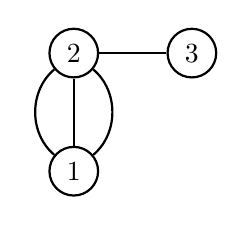
\begin{tikzpicture}[node distance={15mm}, thick, main/.style = {draw, circle}] 
            \node[main] (1) {$1$}; 
            \node[main] (2) [above of=1] {$2$}; 
            \node[main] (3) [right of=2] {$3$}; 

            \draw (1) edge[bend right = 50] (2); 
            \draw (1) -- (2); 
            \draw (1) edge[bend left = 50] (2);
            \draw (2) -- (3);
\end{tikzpicture}\newline\newline
A simple graph is also a multigraph.\newline\newline
\textbf{Definition:}Given a connected multigraph $G = (V, E)$. A cut $C \subseteq E$ is a multiset of edges such that $G' = (V, E \setminus C)$ is not connected.\newline\newline
\textbf{Karger's algorithm (simplified version):}
\begin{enumerate}
    \item Choose an edge at random;
    \item \textit{Contract} the two vertices of that edge;
    \item Repeat until only two vertices remain;
    \item Return the edges between them;
\end{enumerate}
\textbf{Definition:} Given a multigraph $G=(V,E)$ and an edge $e = (u, v)$, the \textbf{contraction} of $G$ with respect to $e$ is: $G_{/e} = (V', E')$ where:
\begin{itemize}
    \item $V' = V \setminus \{u, v\} \cup \{z_{u,v}\}$ where $z_{u,v} \notin V$.

    \item $E' = E \setminus \{\{ (x,y) : (x = u)\,\, \text{or}\,\, (x = v)\}\} \cup \{\{ (z_{u,v}, y) : (u, y) \in E \,\, \text{or} \,\, (v, y) \in E, \,\, y \neq u \,\, \text{and} \,\, y \neq v   \}\}$
\end{itemize}
It follows that:
\begin{itemize}
    \item $|V'| = |V| - 1$

    \item $|E'| = |E| - m(e) \leq |E| - 1$
\end{itemize}
Basically, it makes the two vertices to collapse in just one vertex connected with all the previous adjacent vertices. If as a result there are several edges between some pairs of (newly formed) vertices, retain them all.\newline\newline
\textbf{Example:}\newline\newline
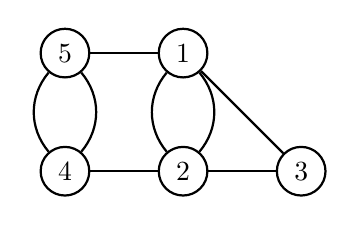
\begin{tikzpicture}[node distance={15mm}, thick, main/.style = {draw, circle}] 
            \node[main] (1) {$1$}; 
            \node[main] (2) [below of=1] {$2$}; 
            \node[main] (3) [right of=2] {$3$};
            \node[main] (4) [left of=2] {$4$};
            \node[main] (5) [above of=4] {$5$}; 

            \draw (1) edge[bend right = 40] (2); 
            \draw (1) edge[bend left = 40] (2);
            \draw (2) -- (3);
            \draw (1) -- (3);
            \draw (5) -- (1);
            \draw (4) -- (2);
            \draw (4) edge[bend right = 40] (5); 
            \draw (4) edge[bend left = 40] (5);
\end{tikzpicture}\newline\newline
The contraction of $G$ with respect to the edge $(1,2)$ is the following:\newline\newline
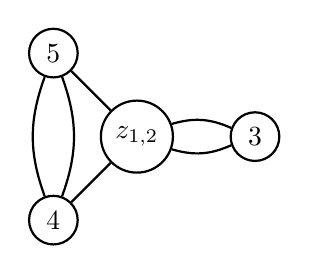
\begin{tikzpicture}[node distance={15mm}, thick, main/.style = {draw, circle}] 
            \node[main] (z) {$z_{1,2}$};
            \node[main] (3) [right of=z] {$3$};
            \node[main] (4) [below left of=z] {$4$};
            \node[main] (5) [above left of=z] {$5$}; 


            \draw (z) edge[bend right = 20] (3);
            \draw (z) edge[bend left = 20] (3);
            \draw (5) -- (z);
            \draw (4) -- (z);
            \draw (4) edge[bend right = 20] (5); 
            \draw (4) edge[bend left = 20] (5);
\end{tikzpicture}\newline\newline
Actually, the probability that at the first run Karger's algorithm returns a minimum cut is \textbf{not} high. The idea is to repeat the procedure $k$ times to reduce the probability of error. The value of $k$ will be determined by the analysis of the algorithm.\newpage
\begin{algorithm}
\caption{Karger's algorithm}\label{KARGER}
    \begin{algorithmic}[1]
    \Procedure{Karger($G, k$)}{}
        \State $min = \infty$
        \For{$i = 1$ to $k$}
            \State $t =$ \textit{FULL\_CONTRACTION($G$)}
            \If{$t < min$}
                \State $min = t$
            \EndIf
        \EndFor
        \Return $min$
    \EndProcedure   
    \end{algorithmic}
\end{algorithm}

\begin{algorithm}
\caption{FULL\_CONTRACTION}\label{FULLC}
    \begin{algorithmic}[1]
    \Procedure{FULL\_CONTRACTION($G = (V, E)$)}{}
        \For{$i = 1$ to $n - 2$}
            \State $e = $ random($E$)
            \State $G' = (V', E') = G_{/e} \quad \text{//Contraction}$
            \State $V = V'$
            \State $E = E'$
        \EndFor
        \Return $|E|$
    \EndProcedure   
    \end{algorithmic}
\end{algorithm}
\section{Analysis of Karger's algorithm}
We'll show for which value of $k$ the algorithm returns a minimum cut with high probability.\newline\newline
\textbf{Property:} $\forall$ cut $C'$ in $G_{/e}$ $\exists$ a cut $C$ in $G$ of the same cardinality.\newline\newline
This implies that $|\text{minimum cut in }G_{/e}| \geq |\text{minimum cut in } G|$.\newline\newline
\textbf{Proof:}Given a cut $C'$ in $G_{/e}$, the idea is to determine the corresponding cut $C$ in $G$ by substituting each edge $(z_{u, v}, y)$ in $C'$ with $(u, y)$ or $(v, y)$. Then, it remains to show that $C$ is a cut in $G$.\newline\newline
Let $C'$ be a cut in $G_{/e} = (V', E')$. Then, $C'$ separates $V'$ in 2 connected components. Let $V_1 \subset V'$ the connected component containing $z_{u,v}$, and let $x \notin V_1$. Then, in $G_{/e}$ every path from $z_{u, v}$ to $x$ must use an edge in $C'$.\newline\newline
Now we'll show that $C$ in $G$ disconnects $u$ and $v$ from $x$. Assume by contradiction that $C$ is \textbf{not} a cut in $G$. This implies that it exists a path between $u$ and $x$ after the removal of $C$ from $E$. Then, the path between $z_{u, v}$ and $x$ \textit{survives} the removal of $C'$ in $G_{/e}$. This implies that $C'$ is not a cut in $G_{/e} \rightarrow$ contradiction!\newline\newline
Note that the cuts that disappear in the contracted graph are the ones hit by the random choice of the edge $e$, all the others are preserved. This means that the only time the algorithm fails is when an edge belonging to a minimum cut in $G$ is hit by the random choice. Basically, by proving the property above we have shown that, if the algorithm never hits an edge belonging to a minimum cut, then it returns a correct solution (because the minimum cut is preserved in $G_{/e}$).\newline\newline
Therefore, we want the probability of \textbf{not} hitting edges of the minimum cut to be sufficiently high.

\subsection{Conditional probability recall}
\textbf{Definition:} The events $E_1, E_2$ are \textbf{independent} if:
\[P(E_1 \cap E_2) = P(E_1) \cdot P(E_2)\]
\textbf{Definition:} Given $P(E_1) > 0$, then:
\[P(E_2 | E_1) = \frac{P(E_1 \cap E_2)}{P(E_1)}\]
extension to $k$ events:
\[P(E_1 \cap E_2 \cap E_3 \cap ... \cap E_k) = P(E_1)P(E_2 | E_1)P(E_3 | E_1 \cap E_2) ... P(E_k | E_1 \cap ... \cap E_{k-1})\]

\subsection{Analysis of \textit{FULL\_CONTRACTION}}
\textbf{Intuition:} Since $|\text{min. cut}|$ is a small portion of $|E|$, it is \textit{unlikely} to hit an edge of a minimum cut. Let's calculate what is this probability.\newline\newline
\textbf{Property:} Let $G=(V, E), \,\, |V| = n$. If $G$ has a minimum cut of size $t$, then $|E| \geq t \cdot \frac{n}{2}$.\newline\newline
\textbf{Proof:} $d(v) \geq t \,\, \forall v \in V$. This is because If we take a node and remove all the edges incident to that node, that's a cut.
\[
    \begin{split}
        \sum_{v \in V}d(v) & = 2m \geq t \cdot n\\
        m & = |E| \geq \frac{t \cdot n}{2}
    \end{split}
\]
Let $t = |\text{minimum cut}|$. Given the event $E_i = \text{in the i-th contruction i did \textbf{not} hit an edge of the minimum cut}$, it follows that:
\[
    \begin{split}
        P(\overline{E}_1) & = \frac{t}{|E|} \leq \frac{t}{t \cdot \frac{n}{2}} = \frac{2}{n}\\
        P(\overline{E}_1) & \leq \frac{2}{n}\\
        P(E_1) & \geq 1 - \frac{2}{n}\\
    \end{split}
\]
Since after every contruction $|V'| = |V| - 1$, the following holds:
\[
    \begin{split}
        P(E_2 | E_1) & \geq 1 - \frac{t}{t \cdot \frac{(n - 1)}{2}} = 1 - \frac{2}{n - 1}\\
        & ... \\
        P(E_i | E_1 \cap ... \cap E_{i-1}) & \geq 1 - \frac{t}{\frac{t(n- i + 1)}{2}} = 1 - \frac{2}{n - i + 1}
    \end{split}
\]
Therefore, the probability that \textit{FULL\_CONTRUCTION} succeeds becomes:
\[
    \begin{split}
        P(\textit{FULL\_CONTRUCTION succeeds}) & \geq P(\bigcap_{i = 1}^{n-2}E_i) = \prod_{i = 1}^{n - 2}\left(1 - \frac{2}{n - i + 1}\right) = \prod_{i = 1}^{n-2} \frac{n - i -1}{n - i + 1}\\
        & \geq \frac{\cancel{n - 2}}{n} \cdot \frac{\cancel{n - 3}}{n - 1} \cdot \frac{\cancel{n - 4}}{\cancel{n - 2}} \cdot\cdot\cdot \frac{\cancel{3}}{\cancel{5}}\cdot\frac{2}{\cancel{4}}\cdot\frac{1}{\cancel{3}} = \frac{2}{n(n - 1)}
    \end{split}
\]
Basically, the probability that \textit{FULL\_CONTRUCTION} does not hit an edge of a minimum cut is at least $\frac{2}{n^2}$. Not so good as a bound. Our algorithm may err
in declaring the cut it outputs to be a min-cut. Karger's amplifies this probability by repeating \textit{FULL\_CONTRUCTION} multiple times:
\[P(\textit{the k runs of FULL\_CONTRUCTION do not return the minimum cut}) \leq \left(1 - \frac{2}{n^2}\right)^{k}\]
We want to find a value for $k$ such that $\left(1 - \frac{2}{n^2}\right)^{k} \leq \frac{1}{n^d}$. In order to do this, we'll use the following two rules:
\begin{itemize}
    \item $(1 + \frac{x}{y})^y \leq e^x \,\, y \geq 1, y \geq x$
    \item $e^{-ln\,n} = \frac{1}{n}$
\end{itemize}
By choosing $k = d\frac{n^2}{2}ln\,n$, it follows that:
\[
    \begin{split}
        & = \left(\left(1 - \frac{2}{n^2}\right)^{n^2}\right)^{\frac{d}{2}ln\, n}\\
        & \leq (e^{-2})^{\frac{d}{2}ln\, n} = e^{-ln\, n^d} = \frac{1}{n^d}
    \end{split}
\]
Then, by choosing that value for $k$ the Karger's algorithm succeeds with high probability:
\[P(\textit{Karger's succeeds}) \geq 1 - \frac{1}{n^d}\]

\subsection{Complexity}
\textit{FULL\_CONTRUCTION} can be implemented in $O(n^2)$. Then, the complexity of Karger's algorithm is $O(n^4log\, n)$. It is not very fast, but it can be improved to obtain a complexity of $O(n^2log^3\,n)$.\newline\newline
The fastest algorithm for this problem has a complexity of $O(m log\,n)$.

\chapter{Lec 21 - Autoencoders}

\section{Autoencoder - General Idea}
Autoencoders (AEs) are an unsupervised learning technique based on feed forward neural networks. The aim of autoencoders is to learn a representation (often called encoding or code) for a set of data, typically for the purpose of dimensionality reduction.\newline\newline
In particular, an autoencoder is a neural network that is trained to attempt to copy its input to its output.  Internally, it has a hidden layer $\textbf{h}$ that describes a code used to represent the input. The network may be viewed as consisting of two parts:
\begin{itemize}
    \item An \textbf{encoder} function $\textbf{h} = f(\textbf{x})$
    \item A \textbf{decoder} function that produces a reconstruction $\textbf{r} = g(\textbf{h})$
\end{itemize}
Since it is not useful to learn the identity function on the whole input domain (hidden code dimension equal to input dimension), autoencoders are trained to learn $\textbf{x} = g(f(\textbf{x}))$ with constraints:
\begin{itemize}
    \item on the architecture of the network (\textbf{undercomplete autoencoder}).

    \item adding a regularizing term to the loss (\textbf{overcomplete autoencoder})
\end{itemize}
Usually they are restricted in ways that allow them to copy only approximately. Because the model is forced to prioritize which aspects of the input should be copied, it often learns \textbf{useful properties} of the data.\newline\newline
Modern autoencoders have generalized the idea of an encoder and a decoder beyond deterministic functions to stochastic mappings $p_{encoder}(\textbf{h} | \textbf{x})$ and $p_{decoder}(\textbf{x} | \textbf{h})$. we may think of the decoder as providing a conditional distribution $p_{decoder}(\textbf{x} | \textbf{h})$. We may then train the autoencoder by minimizing $-log\, p_{decoder}(\textbf{x}|\textbf{h})$.

\section{Undercomplete Autoencoders}
One way to obtain useful features from the autoencoder is to constrain $\textbf{h}$ to have smaller dimension than $\textbf{x}$. An autoencoder whose code dimension is less than the input dimension is called \textbf{undercomplete}. Learning an undercomplete representation forces the autoencoder to capture the most salient features of the training data.\newline\newline
The learning process is described simply as minimizing a loss function;
\[L(\textbf{x}, g(f(\textbf{x}))\]
where $L$ is a loss function penalizing $g(f(\textbf{x}))$ for being dissimilar from $\textbf{x}$, such as the mean squared error.\newline\newline
When the decoder is linear and $L$ is the mean squared error, an undercomplete autoencoder learns to span the same subspace as \textbf{PCA} (SVD). Autoencoders with nonlinear encoder functions $f$ and nonlinear decoder functions $g$ can thus learn a more powerful nonlinear generalization of PCA. However, if the encoder and decoder are allowed too much capacity, the autoencoder can learn to perform the copying task without extracting useful information about the distribution of the data.\newline\newline
Autoencoders are often trained with only a single layer encoder and a single layer
decoder. However, this is not a requirement. In fact, using deep encoders and
decoders offers many advantages. Depth can exponentially reduce the computational cost of representing some functions. Depth can also exponentially decrease the amount of training data needed to learn some functions. Experimentally, \textbf{deep autoencoders} yield much better compression than corresponding shallow or linear autoencoders.

\subsection{Singular Value Decomposition (SVD)}
Singular Value Decomposition (SVD) is a standard linear dimensionality reduction method which combines the features of the original high-dimensional dataset and project them into a lower-dimensional space, ideally retaing most of their intrinsic properties.\newline\newline
Given a matrix $X$, the SVD decomposes it into the product of two unitary matrices, $V$ and $U$, and a rectangular diagonal matrix of singular values $S$:
\[X=V \cdot S \cdot U^T\]
The values in $S$ are called singular values. We can choose to keep only the first $k$ singular values in order to reduce the dimensionality of the input while minimizing the information loss.

\section{Overcomplete Autoencoders}
\textbf{Overcomplete} autoencoders have the hidden code dimension greater than the input. However, autoencoders may fail to learn useful properties of data if the dimension of the code $\textbf{h}$ is greater or equal to the input dimension. Therefore, rather than limiting the model capacity by keeping the encoder and decoder shallow and the code size small, \textbf{regularized autoencoders} use a loss function that encourages the model to have other properties besides the ability to copy its input to its output.\newline\newline
There are different types of regularized autoencoders:
\begin{itemize}
    \item Sparse autoencoders
    \item Denoising autoencoders 
    \item Contractive autoencoders
    \item Autoencoders with Dropout on the hidden layer
\end{itemize}

\section{Sparse Autoencoders}
A sparse autoencoder limits the capacity of the model by adding a sparsity penalty $\Omega(\textbf{h})$ on the code layer $\textbf{h}$, to the cost function:
\[L(\textbf{x}, g(f(\textbf{x}))) + \Omega(\textbf{h})\]
The sparsity penalty makes the model able to perform feature selection. In this way, a sparse autoencoder does not learn just the identity function, but it can learn useful features of the input.\newline\newline
Rather than thinking of the sparsity penalty as a regularizer for the copying task, we can think of the entire sparse autoencoder framework as approximating maximum likelihood training of a generative model that has latent variables (see slides for more details).

\section{Denoising Autoencoders}
Traditionally, autoencoders minimize some function:
\[L(\textbf{x}, g(f(\textbf{x})))\]
A \textbf{denoising autoencoder} or DAE instead minimizes:
\[L(\textbf{x}, g(f(\Tilde{\textbf{x}})))\]
where $\Tilde{\textbf{x}}$ is is a copy of $\textbf{x}$ that has been corrupted by some form of noise. Basically, DAE are forced to reconstruct a corrupted representation of the input. Denoising autoencoders must therefore undo this corruption rather than simply copying their input.\newline\newline
Like many other machine learning algorithms, autoencoders exploit the idea
that data concentrates around a low-dimensional \textbf{manifold}. Autoencoders aim to learn the structure of the manifold.
\begin{center}
    \includegraphics[scale=0.6]{images/manifold.png}
\end{center}

\section{Contractive Autoencoders}
The \textbf{contractive autoencoder} introduces an explicit regularizer on the code $\textbf{h} = f(\textbf{x})$, encouraging the derivatives of $f$ to be as small as possible:
\[\Omega(\textbf{h}) = \lambda ||\frac{\partial f(\textbf{x})}{\partial \textbf{x}}||^2_F\]
The penalty $\Omega(\textbf{h})$ is the squared Frobenius norm (sum of squared elements) of the Jacobian matrix of partial derivatives associated with the encoder function.\newline\newline
This forces the model to learn a function that does not change much when $\textbf{x}$ changes slightly.


\chapter{Lec 22 - Analysis of Randomized Quicksort}

\section{Randomized Quicksort}
\begin{algorithm}
\caption{Randomized Quicksort}\label{RQS}
    \begin{algorithmic}[1]
    \Procedure{RandQuicksort($S$)}{}
        \If{$|S| \leq 1$}
            \Return $S$
        \EndIf
        \State $p = \text{random($S$)}\quad \text{// pick a pivot element uniformly at random from $S$}$
        \State $S_1 = \{x \in S\,\, \text{s.t. }x < p\}$
        \State $S_2 = \{x \in S\,\, \text{s.t. } x > p\}$
        \State $z_1 = RandQuicksort(S_1)$
        \State $z_2 = RandQuicksort(S_2)$
        \State \Return $z_1, z_2$
    \EndProcedure   
    \end{algorithmic}
\end{algorithm}
It is a \textit{LAS VEGAS} algorithm (we choose the pivot at random).\newline\newline
Suppose that $p$ is always the median of $S$, then:
\[
    T_{RQS}(n) = 
    \begin{cases}
        2T_{RQS}(\frac{n}{2}) + O(n) & n > 1 \\
        0 & n\leq 1
    \end{cases}
\]
where $n = |S|$. Then $T_{RQS}(n) = O(nlog\,n)$.\newline\newline
However, $p$ is the median with probability $\frac{1}{n}$, very low. Actually, there exists a deterministic linear algorithm to compute the median. This implies that this version of deterministic Quicksort has complexity $O(nlog\,n)$. The problem is that the hidden constant is very high, thus it is inefficient in practice.\newline\newline
Fortunately, we don't really need that the random choice hits always the median. For example, let's see what happens if the pivot is always chosen between the $(\frac{n}{4} + 1)$-th order statistics and the $(\frac{3}{4}n)$-th order statistics. By looking at the recursion tree, if such a pivot is always chosen, all the root-leaf paths are no longer than $log_{\frac{4}{3}}n$. This is because $|S|$ after $i$ \textit{successes} is $\leq (\frac{3}{4})^in$. This implies that $T_{RQS} = O(nlog\,n)$. It is not necessary that $S_1$ and $S_2$ are perfectly balanced.\newline\newline
If we prove that the depth of the recursion tree is $O(log\,n)$ w.h.p. then $T_{RQS} = O(nlog\,n)$ w.h.p.

\section{Analysis}
Let's call the event $E = \textit{lucky choice of the pivot}$, that is, pivot chosen between the $(\frac{n}{4} + 1)$-th order statistics and the $(\frac{3}{4}n)$-th order statistics. Then:
\[P(E) = \left(\frac{\frac{3}{4} - (\frac{n}{4} + 1) + 1}{n}\right) = \frac{1}{2}\]
Fix \textbf{one} root-leaf path $P_1$:\newline\newline
\textbf{Lemma:} $P(|P_1| > a \cdot log_{\frac{4}{3}}n) < \frac{1}{n^3}$.\newline\newline
If this lemma is true, it follows that:
\begin{enumerate}
    \item Given the event $E_i = \textit{the path $p_i$ has length } > a \cdot log_{\frac{4}{3}}n$:
    \[P(\exists \textit{ a path with length } > a \cdot log_{\frac{4}{3}}n) = P\left(\bigcup_{i=1}^n E_i\right) \leq \sum_{i=1}^n P(E_i) < \frac{1}{n^2}\]

    \item Therefore, the probability that all the root-leaf paths have length $\leq a \cdot log_{\frac{4}{3}}n$ is the following:
    \[P(\textit{all the root-leaf paths have length $\leq a \cdot log_{\frac{4}{3}}n$}) \geq 1 - P(\exists \textit{ a path with length } > a \cdot log_{\frac{4}{3}}n) \geq 1 - \frac{1}{n^2}\]
\end{enumerate}
This would imply that $T_{RQS}(n) = O(nlog\,n)$ w.h.p.\newline\newline
It remains to prove the Lemma above.\newline\newline
\textbf{Proof:} Given a path $\Pi$, let $l = a \cdot log_{\frac{4}{3}}n$. We want to study the event $E =$ \textit{in the first l nodes of $\Pi$ there have been $< log_{\frac{4}{3}}n$ lucky choices}.
\begin{itemize}
    \item $X_i \quad 1 \leq i \leq l$
    \item $X_i = 1$ if at the $i$-th node of $\Pi$ there is a \textit{lucky choice} of the pivot. 
    \item $P(X_i = 1) = \frac{1}{2} \quad \forall i$.
    \item $X_i$ are independent.
\end{itemize}
We want the probability $P(\sum_{i=1}^l X_i) < log_{\frac{4}{3}}n$ to be bound.\newline\newline
Given $X = \sum_{i=1}^l X_i$, its expected value is defined as follows:
\[\mu = E[X] = E\left[\sum_{i=1}^l X_i\right] = \sum_{i=1}^l E[X_i] = \sum_{i=1}^l \frac{1}{2} = \frac{a}{2}log_{\frac{4}{3}}n\]
Now, let's apply the following Chernoff bound:
\[P(X < (1 - d)\mu) < e^{-\mu\frac{d^2}{2}} \quad 0 < d \leq 1\]
We want $(1 - d)\mu = log_{\frac{4}{3}}n$:
\[(1-d)\frac{a}{2}log_{\frac{4}{3}}n = log_{\frac{4}{3}}n\]
One possible solution is:
\begin{itemize}
    \item $a = 8$
    \item $d = \frac{3}{4}$
\end{itemize}
\[
    \begin{split}
        P(X < log_{\frac{4}{3}}n) & < e^{-\frac{8}{4}log_{\frac{4}{3}}n \cdot \frac{9}{16}} \\
        & = e^{-log_{\frac{4}{3}}n\cdot\frac{9}{8}}\\
        & < e^{-log_{\frac{4}{3}}n}\\
        & = e^{-\frac{ln\,n}{ln\,\frac{4}{3}}}\\
        & = \left(e^{-ln\,n}\right)^{\frac{1}{ln\,\frac{4}{3}}}\\
        & = \left(\frac{1}{n}\right)^{1/ln\,\frac{4}{3}}\\
        & < \frac{1}{n^3}
    \end{split}
\]


\end{document}
